\documentclass[../ai_in_finance]{subfiles}
\usepackage[margin=1in]{geometry}
\usepackage{tikz}
\usetikzlibrary{positioning}
\usepackage{amsmath}
\usepackage{amssymb}
\usepackage{booktabs}
\usepackage{floatrow}
\usepackage{draftwatermark}

\SetWatermarkText{WSuo@Queensu.ca}
\SetWatermarkScale{1.4}
\SetWatermarkColor{gray!35}
\SetWatermarkAngle{45}

\usepackage{makeidx}
\makeindex

\begin{document}

\chapter{Machine Learning Fundamentals}

\section{Introduction}

Machine learning has become a central part of the quantitative toolkit in finance. It provides methods for discovering patterns in data, forecasting outcomes, reducing dimensionality, and classifying observations. In principle, its function is simple: use historical data to learn relationships that can generalize to new situations. In practice, this task is not trivial, especially in finance, where data are noisy, relationships shift over time, and the cost of mistakes can be large.

This chapter introduces the main ideas behind machine learning in a way that is accessible to readers who are mathematically trained but may be new to the subject. The focus is on understanding the core concepts, together with the underlying formulas, rather than on memorizing library calls. Two small worked examples run through the chapter: a regression problem relating a firm's leverage to its credit spread, and a classification problem predicting loan default. The discussion covers supervised and unsupervised learning, prediction and classification, overfitting\index{overfitting}, regularization, evaluation strategies, and the bias-variance tradeoff.

By the end of the chapter, the reader will have seen how a model's parameters are actually found (via a closed-form solution or gradient descent\index{gradient descent}), how several qualitatively different algorithms, distance-based, margin-based, probabilistic, and tree-based, all address the same underlying prediction problem from different angles, and how to select among them and their hyperparameters without silently overfitting the selection process itself. These foundations are used directly and repeatedly in every applied chapter that follows: the credit models of Chapter 9, the portfolio methods of Chapter 10, the trading strategies of Chapters 11 and 12, the fraud detection systems of Chapter 13, and the text-based methods of Chapter 14 all build on the vocabulary and techniques introduced here, rather than re-deriving them from scratch.

\section{What Machine Learning Is}\index{What Machine Learning Is}

Suppose an analyst has a decade of loan-application data and wants a system that predicts default risk more accurately than a fixed set of hand-written underwriting rules, one that gets better as more data arrives rather than needing to be manually rewritten every time economic conditions shift. Machine learning is the branch of statistics and computer science built to do exactly this: building models that improve with experience, rather than encoding a fixed decision procedure by hand. The basic setup is straightforward: a model is given data, it learns parameters from those data by minimizing some measure of error, and it is then used to make predictions or decisions on new data. The model may be used for regression, classification, clustering, dimensionality reduction, or anomaly detection.

This basic setup is, in an important sense, not new. Fitting a linear regression by least squares, a technique dating to Gauss and Legendre in the early 1800s, is itself a machine learning algorithm by this definition: it minimizes an error measure (squared error) over a set of parameters using data. What distinguishes the modern field of machine learning is less the underlying mathematical principle, minimizing a loss function over parameters, than the scale of data and computation now available, and the resulting emphasis on flexible, high-capacity models (trees, ensembles, neural networks) whose parameters number in the thousands, millions, or more, and whose behavior is correspondingly harder to interpret than that of the small, transparent linear models classical statistics was built around.

In finance, machine learning can be used for several purposes. It can forecast returns or volatility, classify whether a firm is likely to default, detect fraudulent transactions, or extract sentiment from news articles. The common thread is that the model must learn from observed patterns and then generalize to future cases, which is a fundamentally harder task than simply describing the past.

The challenge is that finance is not a static environment. Relationships can change because of policy shifts, market regimes, investor behavior, or macroeconomic conditions. A model that performs well in one regime may fail in another. This is why machine learning in finance must be approached with care and tested under realistic conditions, a theme that runs throughout this chapter and resurfaces in every applied chapter that follows.

\section{Supervised and Unsupervised Learning}\index{Supervised and Unsupervised Learning}

Machine learning problems are often divided into supervised and unsupervised learning. In supervised learning, the outcome of interest, called the label or target, is observed in the training data. For example, one may have historical data on firm characteristics and a label indicating whether default occurred. The task is to learn a function $\hat f$ mapping features $x$ to a target $y$, so that $\hat f(x) \approx y$ on new, unseen data. Common examples include linear regression, logistic regression\index{logistic regression}, decision trees, and neural networks.

In unsupervised learning, no explicit target is available. The goal is to discover structure in the data. Clustering methods group similar observations together, while dimensionality reduction methods compress the data into lower-dimensional representations. In finance, unsupervised learning can help identify groups of similar assets, detect unusual trading patterns, or reduce the dimensionality of large datasets.

A third category, semi-supervised learning, sits between the two: it uses a small amount of labeled data together with a much larger amount of unlabeled data, which is a common situation in finance where obtaining a reliable label (for example, confirming that a transaction was genuinely fraudulent, which may require a lengthy investigation) is expensive relative to collecting the raw data itself. A related distinction is between discriminative models, which learn the boundary or function that separates or predicts labels directly (linear regression, logistic regression, and most models in this chapter), and generative models, which instead learn the full probability distribution of the data and can be used to generate new, synthetic examples resembling the training data. Naive Bayes\index{Naive Bayes classifier}, introduced later in this chapter, is a simple generative model; large language model\index{large language model (LLM)}s, discussed in Chapter 14, are far more elaborate examples of the same generative principle applied to text.

The distinction is important because the choice of method depends on the question being asked. If one wants to predict default, supervised learning is appropriate. If one wants to understand hidden structure in a large set of securities, unsupervised learning may be more appropriate. The remainder of this chapter proceeds roughly in that order: supervised regression and classification first, since they are the most immediately useful for the applied chapters that follow, then unsupervised clustering and dimensionality reduction, and finally neural networks, which can be applied to either supervised or unsupervised problems depending on how they are trained.

\section{Regression: A Worked Example}\index{Regression: A Worked Example}
\label{sec:regression-example}

Suppose a credit analyst wants to relate a firm's leverage, measured as debt-to-EBITDA, to the credit spread the market demands on its bonds, measured in basis points. Table~\ref{tab:credit_spread_data} shows five observations.

\begin{table}[htbp]
\centering
\caption{Leverage and credit spread for five hypothetical issuers}
\label{tab:credit_spread_data}
\begin{tabular}{lrrrrr}
\toprule
Debt/EBITDA ($x$) & 2 & 3 & 4 & 5 & 6 \\
Credit spread, bps ($y$) & 120 & 150 & 210 & 260 & 300 \\
\bottomrule
\end{tabular}
\end{table}

Linear regression models the target as a linear function of the feature plus noise, $y_i = \beta_0 + \beta_1 x_i + \varepsilon_i$. The ordinary least squares (OLS)\index{Ordinary Least Squares (OLS)} estimator chooses $\beta_0, \beta_1$ to minimize the sum of squared residuals,
\begin{equation*}
(\hat\beta_0, \hat\beta_1) = \arg\min_{\beta_0,\beta_1} \sum_{i=1}^n \left(y_i - \beta_0 - \beta_1 x_i\right)^2,
\end{equation*}
which has the closed-form solution
\begin{equation*}
\hat\beta_1 = \frac{\sum_i (x_i - \bar x)(y_i - \bar y)}{\sum_i (x_i - \bar x)^2}, \qquad \hat\beta_0 = \bar y - \hat\beta_1 \bar x.
\end{equation*}
With $\bar x = 4$ and $\bar y = 208$, the data in Table~\ref{tab:credit_spread_data} give $\sum_i (x_i-\bar x)(y_i - \bar y) = 470$ and $\sum_i (x_i - \bar x)^2 = 10$, so
\begin{equation*}
\hat\beta_1 = \frac{470}{10} = 47, \qquad \hat\beta_0 = 208 - 47(4) = 20.
\end{equation*}
The fitted model is $\widehat{\text{spread}} = 20 + 47 \times \text{leverage}$: each additional turn of debt-to-EBITDA is associated with roughly 47 additional basis points of credit spread. The fitted values are 114, 161, 208, 255, and 302 bps, close to the observed 120, 150, 210, 260, and 300. Figure~\ref{fig:credit_spread_regression} plots the five issuers alongside this fitted line, making the tightness of the fit, and the size of each point's residual, visually immediate.

\begin{figure}[htbp]
\centering
\begin{lrbox}{\bookmeasuredbox}
    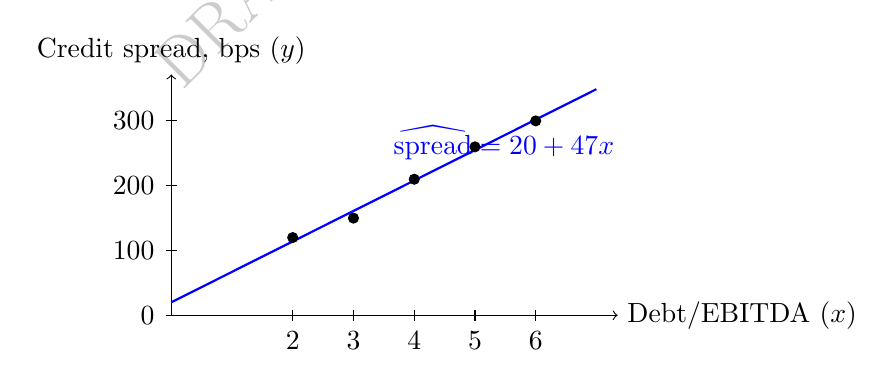
\begin{tikzpicture}[scale=0.9]
        \draw[->] (0,0) -- (6.3,0) node[right] {Debt/EBITDA ($x$)};
        \draw[->] (0,0) -- (0,3.4) node[above] {Credit spread, bps ($y$)};
        \foreach \y/\ylab in {0/0, 0.914/100, 1.829/200, 2.743/300} {
            \draw (-0.08,\y) -- (0.08,\y);
            \node[left] at (-0.1,\y) {\ylab};
        }
        \foreach \x/\xlab in {1.714/2, 2.571/3, 3.429/4, 4.286/5, 5.143/6} {
            \draw (\x,-0.08) -- (\x,0.08);
            \node[below] at (\x,-0.1) {\xlab};
        }
        \draw[thick,blue] (0,0.183) -- (6.0,3.191);
        \foreach \px/\py in {1.714/1.097, 2.571/1.371, 3.429/1.920, 4.286/2.377, 5.143/2.743} {
            \filldraw[black] (\px,\py) circle (2pt);
        }
        \node[above right,blue] at (3.0,2.05) {$\widehat{\text{spread}}=20+47x$};
    \end{tikzpicture}
\end{lrbox}
\ifdim\wd\bookmeasuredbox<0.65\linewidth
\setlength{\bookcapwidth}{0.65\linewidth}
\else
\setlength{\bookcapwidth}{\wd\bookmeasuredbox}
\fi
\ffigbox[\bookcapwidth]{
\usebox{\bookmeasuredbox}
}{
    \caption{Debt-to-EBITDA leverage and credit spread for the five hypothetical issuers in Table~\ref{tab:credit_spread_data} (black dots), with the OLS-fitted line $\widehat{\text{spread}}=20+47x$ overlaid (blue).}
    \label{fig:credit_spread_regression}
}
\end{figure}

The residual sum of squares is
$$\text{SSE} = \sum_i (y_i - \hat y_i)^2 = 190,$$ and the total sum of squares around the mean is
$$\text{SST} = \sum_i (y_i - \bar y)^2 = 22{,}280,$$
giving
\begin{equation*}
R^2 = 1 - \frac{\text{SSE}}{\text{SST}} = 1 - \frac{190}{22{,}280} \approx 0.991,
\end{equation*}
so leverage explains about 99\% of the variation in credit spread in this small, deliberately clean example. In sklearn, the same fit is obtained with

\begin{verbatim}
from sklearn.linear_model import LinearRegression
import numpy as np

X = np.array([2, 3, 4, 5, 6]).reshape(-1, 1)
y = np.array([120, 150, 210, 260, 300])
model = LinearRegression().fit(X, y)
print(model.intercept_, model.coef_)   # 20.0 [47.]
print(model.score(X, y))               # 0.9915...
\end{verbatim}

Real credit spread data would show far more scatter than this toy example; the point is to make the mechanics of fitting and evaluating a linear model completely transparent before adding real-world noise and complexity.

\subsection{Standard Errors, Confidence Intervals, and P-Values for Coefficients}\index{Standard Errors, Confidence Intervals, and P-Values for Coefficients}
\label{sec:regression-inference}

The point estimate $\hat\beta_1 = 47$ says nothing on its own about how confidently the analyst should treat that number, and a machine learning workflow that reports only a point estimate and an $R^2$ is leaving useful information on the table. With $n=5$ observations and two estimated parameters ($\hat\beta_0,\hat\beta_1$), there are $n-2=3$ residual degrees of freedom, and the estimated noise variance is 
$$\hat\sigma^2 = \text{SSE}/(n-2) = 190/3 \approx 63.33.$$
The standard error of the slope, which measures how much $\hat\beta_1$ would be expected to vary across hypothetical repeated samples of five issuers drawn from the same underlying relationship, is
\begin{equation*}
SE(\hat\beta_1) = \sqrt{\frac{\hat\sigma^2}{\sum_i (x_i-\bar x)^2}} = \sqrt{\frac{63.33}{10}} \approx 2.52.
\end{equation*}
Dividing the estimate by its standard error gives the $t$-statistic, $t = 47/2.52 \approx 18.68$, which under the null hypothesis $H_0: \beta_1 = 0$ (leverage carries no information about credit spread at all) follows a $t$-distribution with $3$ degrees of freedom. The associated $p$-value, the probability of observing a $t$-statistic this extreme purely by chance if $H_0$ were true, is $p \approx 0.0003$, far below the conventional $5\%$ threshold; this is strong evidence, within this small and deliberately clean sample, that the slope is genuinely nonzero. A 95\% confidence interval for the slope is
\begin{equation*}
\hat\beta_1 \pm t^*_{0.975,3}\cdot SE(\hat\beta_1) = 47 \pm (3.182)(2.52) \approx (39.0,\ 55.0),
\end{equation*}
using the $t$-distribution critical value $t^*_{0.975,3}\approx 3.182$. The correct reading is that if this sampling and estimation procedure were repeated many times, about $95\%$ of the resulting intervals would contain the true relationship between leverage and spread, not that there is a $95\%$ chance the true $\beta_1$ falls in this specific interval. Applying the same steps to the intercept gives $SE(\hat\beta_0) \approx 10.68$, $t \approx 1.87$, and $p \approx 0.158$: the intercept is not statistically distinguishable from zero at the $5\%$ level, which is unsurprising given that only one of the five leverage values ($x=2$) is anywhere near $x=0$, so the data are not very informative about the spread a zero-leverage issuer would command.

This distinction between the slope's overwhelming significance and the intercept's weak significance illustrates a point that generalizes well beyond this example: statistical significance is coefficient-specific, and a model can pin down some relationships in the data far more precisely than others. It is also worth flagging the same overfitting connection raised throughout this chapter: fitting a regression with many candidate features and reporting only the ones whose $p$-values happen to fall below $0.05$ overstates the evidence, since testing enough coefficients against noise will eventually produce a spuriously ``significant'' one by chance alone, exactly the multiple-testing concern revisited in Chapter 7's discussion of pairs selection for cointegration\index{cointegration} trading. A single small $p$-value is far more persuasive when it was the only hypothesis tested than when it is the best of dozens.

\section{How Models Learn: Gradient Descent}\index{How Models Learn: Gradient Descent}
\label{sec:gradient-descent}

The closed-form OLS solution above exists because linear regression's loss function has a special structure: it is quadratic in the parameters, so its minimum can be found in one step by solving a system of linear equations. Most machine learning models, including logistic regression, neural networks, and many others introduced later in this chapter, do not have this convenient property, and their parameters must instead be found iteratively using an optimization algorithm called gradient descent.

\begin{figure}[htbp]
\centering
\begin{lrbox}{\bookmeasuredbox}
    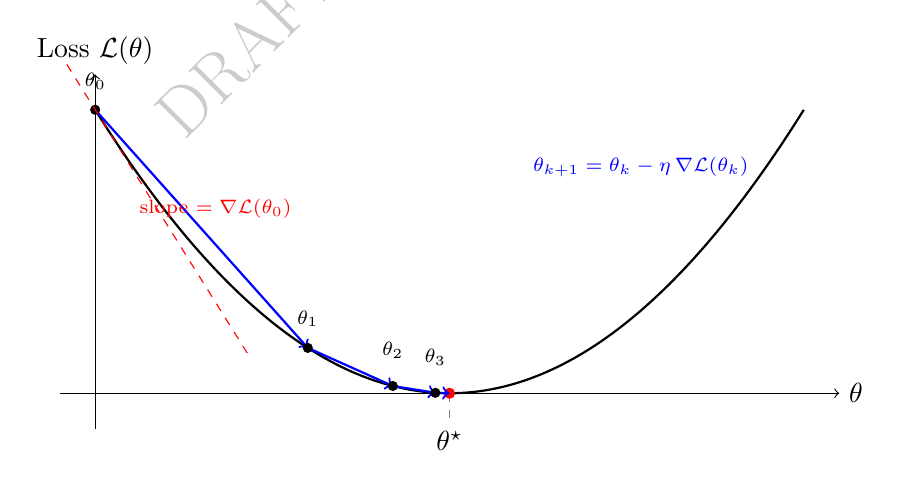
\begin{tikzpicture}[scale=0.9]
        \draw[->] (-0.5,0) -- (10.5,0) node[right] {$\theta$};
        \draw[->] (0,-0.5) -- (0,4.5) node[above] {Loss $\mathcal{L}(\theta)$};
        \draw[thick,domain=0:10,smooth,samples=60,variable=\x] plot ({\x},{0.16*(\x-5)*(\x-5)});
        \draw[dashed,gray] (5,0) -- (5,-0.35);
        \node[below] at (5,-0.4) {$\theta^\star$};
        \filldraw[red] (5,0) circle (2pt);
        \draw[->,thick,blue] (0,4.0) -- (3.0,0.64);
        \draw[->,thick,blue] (3.0,0.64) -- (4.2,0.1024);
        \draw[->,thick,blue] (4.2,0.1024) -- (4.8,0.0064);
        \draw[->,thick,blue] (4.8,0.0064) -- (5.0,0);
        \foreach \px/\py in {0/4.0, 3.0/0.64, 4.2/0.1024, 4.8/0.0064} {
            \filldraw[black] (\px,\py) circle (1.8pt);
        }
        \node[above,font=\scriptsize] at (0,4.15) {$\theta_0$};
        \node[above,font=\scriptsize] at (3.0,0.8) {$\theta_1$};
        \node[above,font=\scriptsize] at (4.2,0.35) {$\theta_2$};
        \node[above,font=\scriptsize] at (4.8,0.25) {$\theta_3$};
        \draw[dashed,red,domain=-0.4:2.2,variable=\x] plot ({\x},{4.0-1.6*\x});
        \node[red,font=\scriptsize] at (1.7,2.6) {slope $=\nabla\mathcal{L}(\theta_0)$};
        \node[blue,font=\scriptsize,align=left] at (7.7,3.2) {$\theta_{k+1} = \theta_k - \eta\,\nabla\mathcal{L}(\theta_k)$};
    \end{tikzpicture}
\end{lrbox}
\ifdim\wd\bookmeasuredbox<0.65\linewidth
\setlength{\bookcapwidth}{0.65\linewidth}
\else
\setlength{\bookcapwidth}{\wd\bookmeasuredbox}
\fi
\ffigbox[\bookcapwidth]{
\usebox{\bookmeasuredbox}
}{
    \caption{The idea of gradient descent. Starting from an initial guess $\theta_0$, each step moves against the local slope of the loss curve, the negative gradient, illustrated here by the tangent line at $\theta_0$, producing a sequence $\theta_0,\theta_1,\theta_2,\ldots$ that descends toward the minimizer $\theta^\star$. Steps are large where the curve is steep and shrink automatically as the curve flattens near the minimum, exactly the pattern seen numerically in Table~\ref{tab:gradient_descent} below.}
    \label{fig:gradient_descent_bowl}
}
\end{figure}

The idea is simple: starting from some initial guess for the parameters, repeatedly take a small step in the direction that most reduces the loss, the negative of the gradient (the vector of partial derivatives) of the loss with respect to each parameter, and stop once further steps no longer improve the loss. For the mean squared error loss 
$$\mathcal{L}(\beta_0, \beta_1) = \frac{1}{n}\sum_i (\beta_0 + \beta_1 x_i - y_i)^2,$$ 
the gradients are
\begin{equation*}
\frac{\partial \mathcal{L}}{\partial \beta_0} = \frac{2}{n}\sum_i (\hat y_i - y_i), \qquad \frac{\partial \mathcal{L}}{\partial \beta_1} = \frac{2}{n}\sum_i (\hat y_i - y_i)\, x_i,
\end{equation*}
and each iteration updates the parameters by
\begin{equation*}
\beta_0 \leftarrow \beta_0 - \eta \frac{\partial \mathcal{L}}{\partial \beta_0}, \qquad \beta_1 \leftarrow \beta_1 - \eta \frac{\partial \mathcal{L}}{\partial \beta_1},
\end{equation*}
where $\eta$ is the learning rate, a small positive number controlling the step size. Applying this to the same credit-spread data as Section~\ref{sec:regression-example}, starting from $\beta_0=\beta_1=0$ with a learning rate of $\eta=0.01$, produces the trajectory in Table~\ref{tab:gradient_descent}.

\begin{table}[htbp]
\centering
\caption{Gradient descent converging toward the closed-form OLS solution}
\label{tab:gradient_descent}
\begin{tabular}{lrr}
\toprule
Iteration & $\beta_0$ & $\beta_1$ \\
\midrule
1      & 4.16  & 18.52 \\
2      & 6.76  & 30.04 \\
3      & 8.38  & 37.21 \\
10     & 11.05 & 48.55 \\
1{,}000   & 18.91 & 47.24 \\
10{,}000  & 20.00 & 47.00 \\
\bottomrule
\end{tabular}
\end{table}


After 10,000 iterations, gradient descent has converged to $\beta_0 \approx 20.00$ and $\beta_1 \approx 47.00$, matching the closed-form OLS solution computed directly in Section~\ref{sec:regression-example} up to rounding. This convergence is not a coincidence: for a quadratic loss function like this one, gradient descent is mathematically guaranteed to converge to the same global minimum that the closed-form formula finds directly, provided the learning rate is small enough to avoid overshooting.

The learning rate itself involves a tradeoff that recurs throughout machine learning: too small, and convergence (as seen here) can require many thousands of iterations; too large, and the updates can overshoot the minimum and diverge rather than converge at all.

In practice, $\eta$ is one of the most important hyperparameters to tune when training a model with gradient descent, including the neural networks discussed later in this chapter, and it is rarely fixed at a single value throughout training; adaptive variants that shrink the learning rate over time, or that use different effective rates for different parameters, are standard in modern deep learning software.

The value of understanding gradient descent, even for a problem like linear regression where a closed-form solution already exists, is that the same algorithm scales to problems with no closed-form solution at all: logistic regression's log-loss, a neural network's loss function with millions of parameters, and many other models throughout this book are all fit using gradient descent or a close variant of it, making it arguably the single most important algorithm in modern machine learning.

\section{Classification: A Worked Example}\index{Classification: A Worked Example}
\label{sec:classification-example}

Regression predicts a continuous target; classification predicts a discrete one, such as whether a borrower defaults. Logistic regression models the probability of the positive class as
\begin{equation*}
p(x) = \Pr(y=1 \mid x) = \frac{1}{1 + e^{-(\beta_0 + \beta_1 x)}},
\end{equation*}
so that $p(x)$ is always between 0 and 1, unlike a linear model's unbounded output. The parameters are typically chosen to minimize the log-loss (negative log-likelihood),
\begin{equation*}
\mathcal{L}(\beta) = -\frac{1}{n}\sum_{i=1}^n \Big[y_i \log p(x_i) + (1-y_i)\log\big(1-p(x_i)\big)\Big].
\end{equation*}
Suppose a lender scores 10 loan applicants and, after choosing a probability threshold, classifies each as predicted default (1) or predicted no default (0). Table~\ref{tab:confusion_data} shows the actual and predicted outcomes.

\begin{table}[htbp]
\centering
\caption{Actual versus predicted default for 10 loan applicants}
\label{tab:confusion_data}
\begin{tabular}{lcccccccccc}
\toprule
Applicant & 1 & 2 & 3 & 4 & 5 & 6 & 7 & 8 & 9 & 10 \\
\midrule
Actual default    & 1 & 0 & 1 & 0 & 0 & 1 & 0 & 0 & 1 & 0 \\
Predicted default & 1 & 0 & 1 & 1 & 0 & 1 & 0 & 0 & 0 & 0 \\
\bottomrule
\end{tabular}
\end{table}

Comparing the two rows produces a confusion matrix\index{confusion matrix}: 3 true positives ($TP$; applicants 1, 3, 6), 1 false negative ($FN$; applicant 9, an actual default the model missed), 1 false positive ($FP$; applicant 4, a good loan flagged as risky), and 5 true negatives ($TN$). Table~\ref{tab:confusion_matrix} arranges these four counts into the standard $2\times 2$ layout, with the model's predictions as rows and the actual outcomes as columns.

\begin{table}[htbp]
\centering
\begin{lrbox}{\bookmeasuredbox}
\begin{tabular}{lcc}
\toprule
 & \multicolumn{2}{c}{Actual} \\
\cmidrule(l){2-3}
Predicted & Default (1) & No Default (0) \\
\midrule
Default (1) & $TP=3$ & $FP=1$ \\
No Default (0) & $FN=1$ & $TN=5$ \\
\bottomrule
\end{tabular}
\end{lrbox}
\ifdim\wd\bookmeasuredbox<0.65\linewidth
\setlength{\bookcapwidth}{0.65\linewidth}
\else
\setlength{\bookcapwidth}{\wd\bookmeasuredbox}
\fi
\ttabbox[\bookcapwidth]{
\usebox{\bookmeasuredbox}
}{
\caption{Confusion matrix for the 10 loan applicants in Table~\ref{tab:confusion_data}}
\label{tab:confusion_matrix}
}
\end{table}

From these four counts, the standard classification metrics follow directly:
\begin{align*}
\text{Accuracy} &= \frac{TP+TN}{n} = \frac{3+5}{10} = 0.80, \\
\text{Precision} &= \frac{TP}{TP+FP} = \frac{3}{4} = 0.75, \\
\text{Recall (TPR)} &= \frac{TP}{TP+FN} = \frac{3}{4} = 0.75, \\
\text{F1} &= \frac{2 \cdot \text{Precision} \cdot \text{Recall}}{\text{Precision}+\text{Recall}} = 0.75, \\
\text{FPR} &= \frac{FP}{FP+TN} = \frac{1}{6} \approx 0.167.
\end{align*}
Each metric answers a different question. Accuracy answers ``what fraction of predictions were correct overall,'' which can be misleading when defaults are rare, since always predicting ``no default'' would score highly on accuracy while being useless. Precision answers ``of the loans flagged as risky, how many actually defaulted,'' which matters when false positives (turning away good customers) are costly. Recall answers ``of the loans that actually defaulted, how many did the model catch,'' which matters when false negatives (missed defaults) are costly. A receiver operating characteristic (ROC) curve\index{Receiver Operating Characteristic (ROC) Curve} plots the true positive rate against the false positive rate as the classification threshold varies, and the area under this curve (AUC)\index{AUC (Area Under the Curve)} summarizes performance across all thresholds at once, rather than at the single threshold used in Table~\ref{tab:confusion_data}.

\section{$K$-Nearest Neighbors: A Non-Parametric Classifier}\index{K-Nearest Neighbors: A Non-Parametric Classifier}

Logistic regression, like linear regression, is a parametric model: it assumes a specific functional form (a linear combination of features passed through a sigmoid) and estimates a fixed, finite set of parameters. $K$-nearest neighbors\index{K-nearest neighbors (KNN)} (KNN) takes a completely different, non-parametric approach: it makes no assumption about the functional form of the relationship between features and target, and instead classifies a new observation by looking directly at the $k$ most similar observations in the training data and taking a majority vote of their labels.

Consider a small loan-underwriting dataset with two features, debt-to-income ratio (\%) and years of credit history, shown in Table~\ref{tab:knn_data}.

\begin{table}[htbp]
\centering
\caption{A small loan dataset for $K$-nearest neighbors classification}
\label{tab:knn_data}
\begin{tabular}{lrrl}
\toprule
Applicant & Debt/income (\%) & Credit history (yrs) & Outcome \\
\midrule
A & 35 & 2  & Default \\
B & 20 & 8  & No default \\
C & 40 & 1  & Default \\
D & 15 & 10 & No default \\
E & 30 & 3  & Default \\
F & 18 & 7  & No default \\
\bottomrule
\end{tabular}
\end{table}

To classify a new applicant with debt-to-income of 28\% and 4 years of credit history, KNN computes the Euclidean distance from this query point to every training point,
\begin{equation*}
d = \sqrt{(28 - x_1)^2 + (4 - x_2)^2},
\end{equation*}
giving
\begin{align*}
d_E &= 2.24, & d_A &= 7.28, & d_B &= 8.94, \\
d_F &= 10.44, & d_C &= 12.37, & d_D &= 14.32,
\end{align*}
sorted from nearest to farthest. With $k=3$, the three nearest neighbors are E (Default), A (Default), and B (No default), so the majority vote (2 Default, 1 No default) classifies the new applicant as a predicted default. Figure~\ref{fig:knn_geometry} shows this geometrically: the query point sits closest to a mix of Default and No-default points, and only the identity of its $k$ nearest neighbors, not any global decision boundary, determines the prediction.

\begin{figure}[htbp]
\centering
\begin{lrbox}{\bookmeasuredbox}
    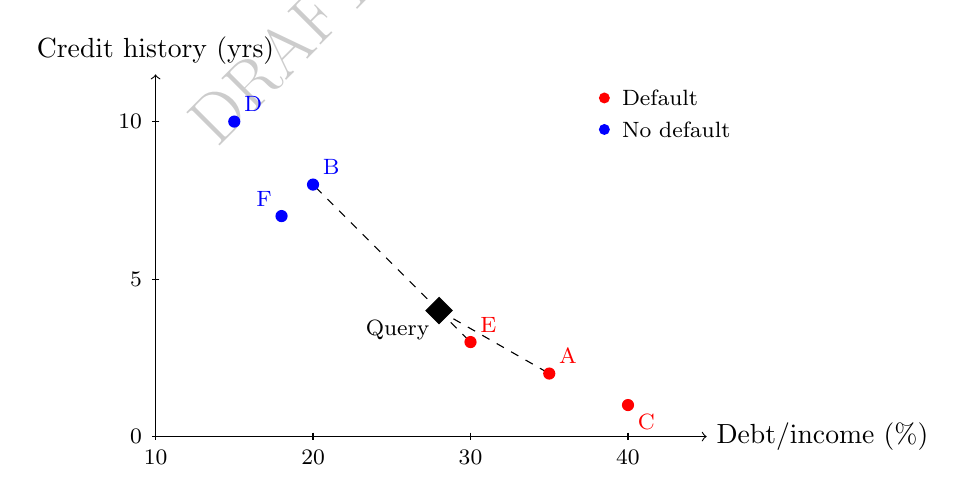
\begin{tikzpicture}[scale=1.0]
        \draw[->] (0,0) -- (7.0,0) node[right] {Debt/income (\%)};
        \draw[->] (0,0) -- (0,4.6) node[above] {Credit history (yrs)};
        \foreach \x/\lbl in {0/10, 2/20, 4/30, 6/40} {
            \draw (\x,0.05) -- (\x,-0.05) node[below,font=\footnotesize] {\lbl};
        }
        \foreach \y/\lbl in {0/0, 2/5, 4/10} {
            \draw (0.05,\y) -- (-0.05,\y) node[left,font=\footnotesize] {\lbl};
        }
        \draw[dashed] (3.6,1.6) -- (4.0,1.2);
        \draw[dashed] (3.6,1.6) -- (5.0,0.8);
        \draw[dashed] (3.6,1.6) -- (2.0,3.2);
        \fill[red] (5.0,0.8) circle (2.2pt) node[above right,font=\footnotesize] {A};
        \fill[blue] (2.0,3.2) circle (2.2pt) node[above right,font=\footnotesize] {B};
        \fill[red] (6.0,0.4) circle (2.2pt) node[below right,font=\footnotesize] {C};
        \fill[blue] (1.0,4.0) circle (2.2pt) node[above right,font=\footnotesize] {D};
        \fill[red] (4.0,1.2) circle (2.2pt) node[above right,font=\footnotesize] {E};
        \fill[blue] (1.6,2.8) circle (2.2pt) node[above left,font=\footnotesize] {F};
        \node[draw,rectangle,rotate=45,minimum size=3pt,fill=black] at (3.6,1.6) {};
        \node[below left,font=\footnotesize] at (3.6,1.6) {Query};
        \node[circle,fill=red,inner sep=1.4pt] at (5.7,4.3) {};
        \node[right,font=\footnotesize] at (5.8,4.3) {Default};
        \node[circle,fill=blue,inner sep=1.4pt] at (5.7,3.9) {};
        \node[right,font=\footnotesize] at (5.8,3.9) {No default};
    \end{tikzpicture}
\end{lrbox}
\ifdim\wd\bookmeasuredbox<0.65\linewidth
\setlength{\bookcapwidth}{0.65\linewidth}
\else
\setlength{\bookcapwidth}{\wd\bookmeasuredbox}
\fi
\ffigbox[\bookcapwidth]{
\usebox{\bookmeasuredbox}
}{
    \caption{The $K$-nearest neighbors example of Table~\ref{tab:knn_data}: six labeled training points and the query applicant (debt/income 28\%, 4 years of credit history, black diamond), with dashed lines to its three nearest neighbors under $k=3$.}
    \label{fig:knn_geometry}
}
\end{figure}

The choice of $k$ controls a bias-variance tradeoff directly analogous to the one in Section~\ref{sec:overfitting-section}: a small $k$ (even $k=1$) makes the prediction highly sensitive to individual nearby points, including noisy or mislabeled ones (high variance), while a large $k$ smooths over local structure and can underfit, in the extreme case where $k$ equals the entire training set, always predicting the overall majority class regardless of the query point (high bias). KNN also has a practical limitation that becomes severe in high dimensions: as the number of features grows, all points tend to become roughly equidistant from one another, a phenomenon known as the curse of dimensionality\index{Curse of Dimensionality}, which is one reason KNN is more commonly used with a small number of carefully chosen features than as a general-purpose model for wide financial datasets.

\section{Support Vector Machines}\index{Support Vector Machines}

Suppose a credit analyst has a single, standardized measure of financial distress for a handful of firms and wants to draw the clearest possible dividing line between the ones that later defaulted and the ones that did not, not just any line that happens to separate the two groups in the historical data, but the one least likely to misclassify a new, slightly different firm sitting close to the boundary. A support vector machine\index{support vector machine (SVM)} (SVM) approaches classification geometrically: rather than modeling a probability (logistic regression) or voting among neighbors (KNN), it searches directly for the hyperplane (a line, in two dimensions) that separates the two classes with the widest possible margin, the distance from the separating boundary to the nearest training point of either class. Intuitively, a wider margin means the decision boundary is less sensitive to small perturbations in the data, which is one reason SVMs often generalize well.

The training points that lie exactly on the margin, the closest points to the boundary, are called support vectors, since they alone determine the position of the separating hyperplane; every other training point could, in principle, be moved or removed without changing the fitted boundary at all, in contrast to a linear regression, where every point contributes to the fitted line. When the classes cannot be separated perfectly by a straight line, a soft-margin SVM allows some points to fall on the wrong side of the margin, controlled by a penalty parameter that trades off margin width against the number of misclassified training points, directly analogous to the regularization strength $\lambda$ in ridge and lasso regression.

SVMs can also be extended to nonlinear decision boundaries using the ``kernel trick,'' which implicitly maps the original features into a higher-dimensional space where a linear separator corresponds to a nonlinear boundary in the original feature space, without ever explicitly computing the higher-dimensional coordinates. In finance, SVMs have historically been used for classification tasks such as bankruptcy prediction and directional price forecasting, though tree-based ensembles (Section~\ref{sec:tree-models}) and neural networks have become more common choices for large, tabular financial datasets in recent years, in part because SVMs scale less gracefully to very large training sets and because tree-based models typically require less feature preprocessing.

A deliberately simple example makes the maximum-margin idea concrete without requiring the full quadratic-programming machinery SVMs use in practice. Suppose four training points are perfectly separable along a single feature (say, a standardized measure of financial distress): two ``high-risk'' points at $x=1$ and $x=2$, and two ``low-risk'' points at $x=4$ and $x=5$. Because the classes are already perfectly separated along this one dimension, the maximum-margin hyperplane is simply the point exactly halfway between the two closest points of opposite classes, $x=2$ and $x=4$, namely $x=3$.

Writing the decision function as $w x + b$ with $w=1$, the boundary condition $wx+b=0$ at $x=3$ requires $b=-3$, and checking the two nearest points confirms $w(2)+b = 2-3=-1$ and $w(4)+b=4-3=1$, exactly the $\pm 1$ margin boundaries the SVM optimization enforces. The points at $x=2$ and $x=4$ are the support vectors: they alone determine $w$ and $b$, and the geometric margin, the distance from the boundary to either margin boundary, is $1/|w|=1$, for a total margin width of $2$, the full gap between the nearest opposite-class points.

The two more extreme points, $x=1$ and $x=5$, play no role at all in determining the boundary, illustrating concretely the earlier claim that only support vectors matter: moving the point at $x=1$ to $x=-100$ would not change the fitted hyperplane in the slightest, whereas moving the support vector at $x=2$ even slightly would immediately shift the boundary. Figure~\ref{fig:svm_margin} shows this geometry directly.

\begin{figure}[htbp]
\centering
\begin{lrbox}{\bookmeasuredbox}
    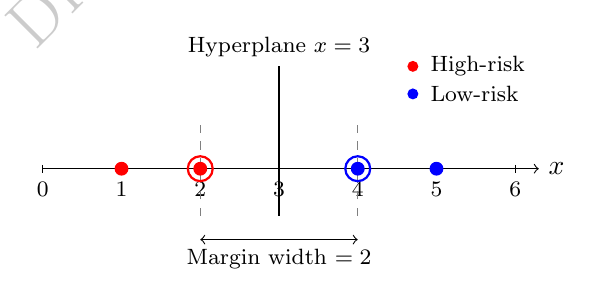
\begin{tikzpicture}[scale=1.0]
        \draw[->] (0,0) -- (6.3,0) node[right] {$x$};
        \foreach \x in {0,1,2,3,4,5,6} {
            \draw (\x,0.05) -- (\x,-0.05) node[below,font=\footnotesize] {\x};
        }
        \draw[dashed,gray] (2,-0.6) -- (2,0.6);
        \draw[dashed,gray] (4,-0.6) -- (4,0.6);
        \draw[thick] (3,-0.6) -- (3,1.3);
        \node[above,font=\footnotesize] at (3,1.3) {Hyperplane $x=3$};
        \draw[<->] (2,-0.9) -- (4,-0.9) node[midway,below,font=\footnotesize] {Margin width $=2$};
        \fill[red] (1,0) circle (2.5pt);
        \draw[red,thick] (2,0) circle (4.5pt);
        \fill[red] (2,0) circle (2.5pt);
        \draw[blue,thick] (4,0) circle (4.5pt);
        \fill[blue] (4,0) circle (2.5pt);
        \fill[blue] (5,0) circle (2.5pt);
        \node[circle,fill=red,inner sep=1.4pt] at (4.7,1.3) {};
        \node[right,font=\footnotesize] at (4.8,1.3) {High-risk};
        \node[circle,fill=blue,inner sep=1.4pt] at (4.7,0.95) {};
        \node[right,font=\footnotesize] at (4.8,0.95) {Low-risk};
    \end{tikzpicture}
\end{lrbox}
\ifdim\wd\bookmeasuredbox<0.65\linewidth
\setlength{\bookcapwidth}{0.65\linewidth}
\else
\setlength{\bookcapwidth}{\wd\bookmeasuredbox}
\fi
\ffigbox[\bookcapwidth]{
\usebox{\bookmeasuredbox}
}{
    \caption{The maximum-margin hyperplane for the one-dimensional example: two high-risk points ($x=1,2$) and two low-risk points ($x=4,5$), with the support vectors circled.}
    \label{fig:svm_margin}
}
\end{figure}

\section{Overfitting and Generalization}\index{Overfitting and Generalization}
\label{sec:overfitting-section}

A central problem in machine learning is overfitting. A complex model can fit the training data very well yet fail when applied to new data. This occurs because the model has learned noise, quirks, or idiosyncrasies that are not repeated outside the sample. In finance, this is especially important because historical data can be highly noisy and because market regimes shift over time. Table~\ref{tab:overfitting_stylized} shows a stylized pattern that recurs constantly in practice: as a model (here, a polynomial regression) is allowed to grow more flexible, training error keeps falling, but test error falls only up to a point and then rises again.

\begin{table}[htbp]
\centering
\caption{Stylized training and test error as model complexity increases}
\label{tab:overfitting_stylized}
\begin{tabular}{lccccc}
\toprule
Polynomial degree & 1 & 2 & 3 & 5 & 9 \\
\midrule
Training error (MSE) & 8.4 & 6.1 & 4.9 & 3.0 & 0.4 \\
Test error (MSE)     & 9.0 & 6.5 & 5.4 & 6.8 & 15.2 \\
\bottomrule
\end{tabular}
\end{table}

The minimum test error in Table~\ref{tab:overfitting_stylized} occurs at degree 3, not at the most flexible model, degree 9, even though degree 9 fits the training data almost perfectly. This gap between training and test performance is the signature of overfitting, and it is the reason a model should never be selected purely on training performance. Figure~\ref{fig:overfitting_curve} plots the same two rows of Table~\ref{tab:overfitting_stylized} as curves rather than numbers, making the characteristic divergence easier to see at a glance.

\begin{figure}[htbp]
\centering
\begin{lrbox}{\bookmeasuredbox}
    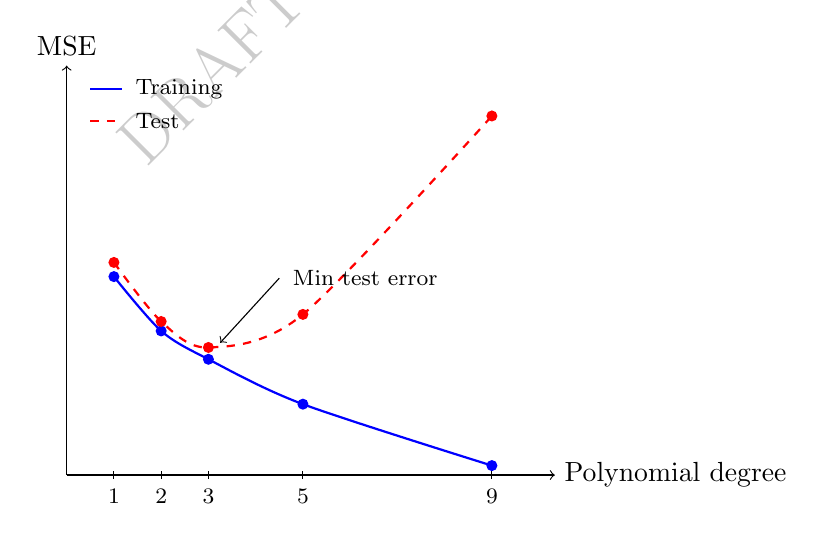
\begin{tikzpicture}[scale=1.0]
        \draw[->] (0,0) -- (6.2,0) node[right] {Polynomial degree};
        \draw[->] (0,0) -- (0,5.2) node[above] {MSE};
        \foreach \x/\lbl in {0.6/1, 1.2/2, 1.8/3, 3.0/5, 5.4/9} {
            \draw (\x,0.05) -- (\x,-0.05) node[below,font=\footnotesize] {\lbl};
        }
        \draw[blue,thick,smooth] plot coordinates {(0.6,2.52) (1.2,1.83) (1.8,1.47) (3.0,0.90) (5.4,0.12)};
        \draw[red,thick,dashed,smooth] plot coordinates {(0.6,2.70) (1.2,1.95) (1.8,1.62) (3.0,2.04) (5.4,4.56)};
        \fill[blue] (0.6,2.52) circle (2pt);
        \fill[blue] (1.2,1.83) circle (2pt);
        \fill[blue] (1.8,1.47) circle (2pt);
        \fill[blue] (3.0,0.90) circle (2pt);
        \fill[blue] (5.4,0.12) circle (2pt);
        \fill[red] (0.6,2.70) circle (2pt);
        \fill[red] (1.2,1.95) circle (2pt);
        \fill[red] (1.8,1.62) circle (2pt);
        \fill[red] (3.0,2.04) circle (2pt);
        \fill[red] (5.4,4.56) circle (2pt);
        \draw[->,thin] (2.7,2.5) -- (1.95,1.68);
        \node[right,font=\footnotesize] at (2.75,2.5) {Min test error};
        \draw[blue,thick] (0.3,4.9) -- (0.7,4.9);
        \node[right,font=\footnotesize] at (0.75,4.9) {Training};
        \draw[red,thick,dashed] (0.3,4.5) -- (0.7,4.5);
        \node[right,font=\footnotesize] at (0.75,4.5) {Test};
    \end{tikzpicture}
\end{lrbox}
\ifdim\wd\bookmeasuredbox<0.65\linewidth
\setlength{\bookcapwidth}{0.65\linewidth}
\else
\setlength{\bookcapwidth}{\wd\bookmeasuredbox}
\fi
\ffigbox[\bookcapwidth]{
\usebox{\bookmeasuredbox}
}{
    \caption{Training and test error (MSE) from Table~\ref{tab:overfitting_stylized} as polynomial degree increases.}
    \label{fig:overfitting_curve}
}
\end{figure}

Generalization refers to the ability of a model to perform on unseen data. The goal of model selection is not merely to maximize performance on the training set, but to choose a model that will perform well out of sample. $k$-fold cross-validation\index{cross-validation} formalizes this: the data are split into $k$ roughly equal parts, and the model is trained on $k-1$ of them and evaluated on the remaining part, repeating $k$ times so that every observation is used for validation exactly once. Figure~\ref{fig:cv} illustrates a single fold of 5-fold cross-validation.

\begin{figure}[htbp]
\centering
\begin{lrbox}{\bookmeasuredbox}
    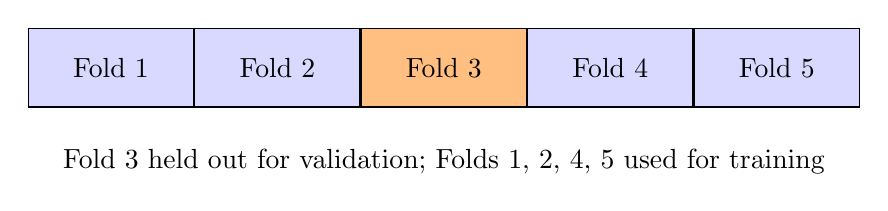
\begin{tikzpicture}[node distance=0mm]
        \node[draw,fill=blue!15,minimum width=2.1cm,minimum height=1cm] (f1) at (0,0) {Fold 1};
        \node[draw,fill=blue!15,minimum width=2.1cm,minimum height=1cm,right=0mm of f1] (f2) {Fold 2};
        \node[draw,fill=orange!50,minimum width=2.1cm,minimum height=1cm,right=0mm of f2] (f3) {Fold 3};
        \node[draw,fill=blue!15,minimum width=2.1cm,minimum height=1cm,right=0mm of f3] (f4) {Fold 4};
        \node[draw,fill=blue!15,minimum width=2.1cm,minimum height=1cm,right=0mm of f4] (f5) {Fold 5};
        \node[below=4mm of f3] {Fold 3 held out for validation; Folds 1, 2, 4, 5 used for training};
    \end{tikzpicture}
\end{lrbox}
\ifdim\wd\bookmeasuredbox<0.65\linewidth
\setlength{\bookcapwidth}{0.65\linewidth}
\else
\setlength{\bookcapwidth}{\wd\bookmeasuredbox}
\fi
\ffigbox[\bookcapwidth]{
\usebox{\bookmeasuredbox}
}{
    \caption{One iteration of 5-fold cross-validation. The procedure repeats five times, holding out a different fold each time, and the five validation scores are averaged.}
    \label{fig:cv}
}
\end{figure}

For financial time series, ordinary $k$-fold cross-validation can be misleading because it may train on future data and validate on the past, which is not possible in real deployment. Walk-forward validation, in which the training window always precedes the validation window in time, is the standard alternative and is discussed further in Chapter 7.

Regularization is a technique designed to reduce overfitting by penalizing model complexity directly in the optimization objective. Ridge regression\index{Ridge Regression} adds a penalty proportional to the sum of squared coefficients,
\begin{equation*}
\hat\beta^{\text{ridge}} = \arg\min_\beta \sum_{i=1}^n (y_i - x_i^\top \beta)^2 + \lambda \sum_{j=1}^p \beta_j^2,
\end{equation*}
while lasso regression\index{Lasso Regression} uses the sum of absolute values,
\begin{equation*}
\hat\beta^{\text{lasso}} = \arg\min_\beta \sum_{i=1}^n (y_i - x_i^\top \beta)^2 + \lambda \sum_{j=1}^p |\beta_j|.
\end{equation*}
In both cases, $\lambda \geq 0$ controls the strength of the penalty: $\lambda = 0$ recovers ordinary least squares, and larger $\lambda$ shrinks coefficients toward zero, trading a small increase in bias for a potentially large reduction in variance. Lasso has the additional property that it can shrink coefficients exactly to zero, which makes it useful for feature selection when many candidate predictors are available, a common situation in finance.

\subsection*{A Worked Example: Ridge Versus Lasso on a Genuine and a Spurious Feature}

The sparsity property is easiest to see with two features, one genuinely predictive and one pure noise, fit with both penalties at the identical $\lambda$. Simulating $200$ observations with $y = 2.0\,x_1 + \varepsilon$, where $x_1$ and $x_2$ are independent standard-normal features and $x_2$ has no relationship to $y$ at all, ordinary least squares correctly identifies both roles, $\hat\beta_1^{\text{OLS}} \approx 1.949$ and $\hat\beta_2^{\text{OLS}} \approx 0.031$, the latter small and attributable to sampling noise alone. Fitting ridge and lasso at the same penalty strength $\lambda=1.0$ gives
\begin{equation*}
\hat\beta^{\text{ridge}} = (1.936,\ 0.030), \qquad \hat\beta^{\text{lasso}} = (0.654,\ 0.000),
\end{equation*}
a striking contrast: ridge barely moves either coefficient at this $\lambda$, while lasso drives the spurious feature's coefficient to \emph{exactly} zero (not merely small) while more aggressively shrinking the genuine feature's coefficient from $1.949$ toward $0.654$. This illustrates lasso's defining behavior directly: rather than shrinking every coefficient smoothly and proportionally the way ridge does, lasso's penalty has a kink at zero that makes it optimal, past a certain threshold, to set a weak coefficient to precisely zero rather than merely small, effectively performing feature selection as a side effect of fitting the model rather than as a separate step. The fact that ridge and lasso require quite different $\lambda$ values to achieve a comparable degree of overall shrinkage, evident from how little this particular $\lambda=1.0$ moved the ridge coefficients, is itself a practical lesson: the two penalties' $\lambda$ values are not interchangeable or directly comparable in magnitude, and each must be tuned separately (for example via the cross-validation procedure introduced earlier in this section) rather than assumed to behave similarly at the same nominal strength.

\section{Bias, Variance, and the Tradeoff}\index{Bias, Variance, and the Tradeoff}
\label{sec:bias-variance}

Suppose two analysts fit different models to the exact same noisy training sample: one fits a single straight line, the other fits a high-degree polynomial that passes through every training point exactly, the degree-9 fit in Table~\ref{tab:overfitting_stylized} among them. Which one should be trusted on new data the model has not yet seen, and why? The bias-variance tradeoff is the foundational concept in machine learning that answers this precisely. For a model $\hat f$ trained on random training data and evaluated at a point $x$ with true relationship 
$$y = f(x) + \varepsilon,$$ 
where $\varepsilon$ has mean zero and variance $\sigma^2$, the expected squared prediction error decomposes as
\begin{equation*}
\mathbb{E}\left[(y - \hat f(x))^2\right] = \underbrace{\left(f(x) - \mathbb{E}[\hat f(x)]\right)^2}_{\text{Bias}^2} + \underbrace{\text{Var}\big(\hat f(x)\big)}_{\text{Variance}} + \underbrace{\sigma^2}_{\text{Irreducible error}}.
\end{equation*}
A model with high bias is too simple and systematically misses the true relationship, regardless of how much data it sees; a straight line fit to a strongly curved relationship is a typical example. A model with high variance is too flexible and reacts strongly to the noise in whatever particular training sample it happened to see; the degree-9 polynomial in Table~\ref{tab:overfitting_stylized} is a typical example. A good model strikes a balance between the two, and this is exactly what the minimum of the test error curve in Table~\ref{tab:overfitting_stylized} represents: the complexity level at which bias and variance are jointly minimized, not the complexity level that minimizes bias alone.

This tradeoff is especially relevant in finance. A very simple model may be stable but fail to capture subtle structure. A very complex model may fit the sample well but fail in real deployment because it does not generalize. With limited data and unstable relationships, simpler, higher-bias models can be surprisingly effective, because their lower variance makes them more robust across changing regimes. With large, high-quality datasets and a stable signal, more complex models may perform better. The key is to evaluate models honestly, using out-of-sample or walk-forward testing, and not assume that complexity automatically improves results.

\section{Hyperparameter Tuning and Model Selection}\index{Hyperparameter Tuning and Model Selection}

Every model introduced in this chapter has at least one hyperparameter, a setting chosen before training rather than learned from the data, that controls its position on the bias-variance spectrum: the ridge penalty $\lambda$, the number of neighbors $k$ in KNN, the maximum depth of a decision tree, or the number of trees and learning rate in a gradient-boosted ensemble. Choosing these hyperparameters well is often as consequential for a model's real-world performance as choosing the model family itself, and it must be done without ever looking at the final test set, or the resulting performance estimate is no longer a trustworthy measure of generalization.

The standard workflow, called grid search combined with cross-validation, proceeds as follows: specify a grid of candidate hyperparameter values (for example, $\lambda \in \{0.01, 0.1, 1, 10, 100\}$), and for each candidate value, run $k$-fold cross-validation (or, for time series data, the walk-forward validation introduced in Chapter 7) entirely within the training set, recording the average validation performance. The hyperparameter value with the best average cross-validated performance is then selected, and only at this point is the model retrained on the full training set and evaluated once on the held-out test set, which was never used during the search. This nested structure, tuning within cross-validation, and only then checking the final test set, is essential: using the test set to choose hyperparameters, even informally by trying a few values and picking the one that looks best on the test set, quietly reintroduces the same overfitting problem that cross-validation was designed to prevent, and inflates the reported performance in a way that will not hold up in production.

Financial applications typically add two further complications to this standard workflow. First, because financial time series exhibit the non-stationarity discussed throughout this book, the hyperparameters selected on one period's data are not guaranteed to remain optimal in a later period, which argues for periodically re-running the tuning process rather than fixing hyperparameters permanently. Second, the grid search itself, trying many hyperparameter combinations, is a form of multiple testing exactly analogous to the backtest-overfitting concern discussed in Chapter 7: searching over a very large grid increases the chance of finding a hyperparameter setting that performs well on the validation folds purely by chance, which is why practitioners often prefer a modest, economically motivated grid over an exhaustive search across hundreds of candidate values.

\section{Model Evaluation}\index{Model Evaluation}

Evaluating a machine learning model requires more than looking at a single number. Different tasks require different metrics. For regression, common metrics include mean squared error (MSE), mean absolute error (MAE), and $R^2$, all illustrated in Section~\ref{sec:regression-example}. For classification, common metrics include accuracy, precision, recall, F1, and AUC, all illustrated in Section~\ref{sec:classification-example}. In finance, one also cares about calibration\index{calibration} (do predicted probabilities match observed frequencies), stability (does performance hold up across different time periods), and economic usefulness (does the model's output translate into a profitable or risk-reducing decision after costs).

A model that predicts default with high accuracy may still be impractical if it is poorly calibrated, produces too many false positives, or fails to distinguish risk levels in a useful way. Likewise, a trading model may have good statistical performance but poor economic performance once transaction costs and execution limits are considered. This is why evaluation in finance must be tied to the actual decision problem, not just to a generic statistical scorecard.

Calibration deserves a brief numerical illustration since it is easy to confuse with accuracy. Suppose a credit model assigns a predicted default probability of $20\%$ to a group of 50 borrowers. The model is well calibrated for this group if, among those 50 borrowers, close to 10 (that is, $20\% \times 50$) actually default; if instead only 2 default, the model's probabilities are too high (poorly calibrated) even if the model still ranks borrowers correctly from most to least risky, which is exactly the kind of distinction accuracy and even AUC can miss, since both depend only on the ranking of predictions, not on whether the predicted probabilities themselves are numerically meaningful. Calibration matters enormously in finance because predicted probabilities are frequently used directly in downstream calculations, such as the expected-loss and reserve calculations in Chapter 9, where a systematically overstated or understated default probability translates directly into an overstated or understated dollar reserve, not just a misranked list of borrowers.

\section{Practical Considerations in Financial ML}\index{Practical Considerations in Financial ML}

The practical deployment of machine learning in finance requires attention to data leakage, sample selection, and concept drift. Data leakage\index{Data Leakage} occurs when information that would not be available at prediction time is used in the model, for example including a variable that is only recorded after the outcome is known. This can produce optimistic in-sample or backtest results that vanish once the model is used in real time. Sample selection issues arise when the training data are not representative of the future environment, for instance training a credit model only on approved loans, which excludes information about applicants who were rejected. Concept drift\index{Concept Drift} occurs when the relationship between features and outcomes changes over time, for example when a recession changes which borrower characteristics matter most for default.

A compact view of the modeling lifecycle is shown in Figure~\ref{fig:ml_lifecycle}.

\begin{figure}[htbp]
\centering
\begin{lrbox}{\bookmeasuredbox}
    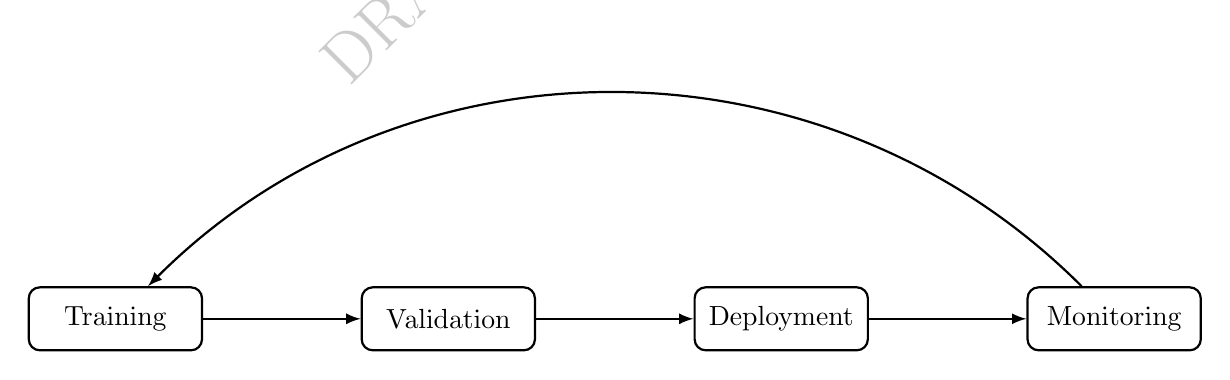
\begin{tikzpicture}[>=latex,thick,node distance=2.0cm]
        \node[draw,rounded corners,minimum width=2.2cm,minimum height=0.8cm] (train) {Training};
        \node[draw,rounded corners,minimum width=2.2cm,minimum height=0.8cm,right=of train] (validate) {Validation};
        \node[draw,rounded corners,minimum width=2.2cm,minimum height=0.8cm,right=of validate] (deploy) {Deployment};
        \node[draw,rounded corners,minimum width=2.2cm,minimum height=0.8cm,right=of deploy] (monitor) {Monitoring};
        \draw[->] (train) -- (validate);
        \draw[->] (validate) -- (deploy);
        \draw[->] (deploy) -- (monitor);
        \draw[->] (monitor) to[out=135,in=45] (train);
    \end{tikzpicture}
\end{lrbox}
\ifdim\wd\bookmeasuredbox<0.65\linewidth
\setlength{\bookcapwidth}{0.65\linewidth}
\else
\setlength{\bookcapwidth}{\wd\bookmeasuredbox}
\fi
\ffigbox[\bookcapwidth]{
\usebox{\bookmeasuredbox}
}{
    \caption{A machine learning workflow in finance should include training, validation, deployment, and continuous monitoring, with findings from monitoring feeding back into retraining.}
    \label{fig:ml_lifecycle}
}
\end{figure}

These issues are not minor technicalities. They often determine whether a model survives in production. Strong financial modeling involves not only fitting a statistical relationship, but also ensuring that the relationship is stable enough to remain useful, and building the monitoring infrastructure to detect when it stops being useful.

\section{Feature Engineering for Financial Data}\index{Feature Engineering for Financial Data}

Every model in this chapter takes a fixed set of numerical features as input, but raw financial data, prices, financial statement line items, transaction records, are rarely usable directly, and the process of transforming raw data into informative model inputs, called feature engineering, is often as important to a model's performance as the choice of algorithm itself.

Several patterns recur constantly when engineering features from financial data. Ratios, such as the debt-to-equity and margin ratios computed throughout Chapter 4, normalize raw dollar figures so that firms of very different sizes become comparable, exactly as the common-size statements in that chapter did.

Lagged and rolling features, such as a 30-day rolling volatility or a 12-month trailing revenue growth rate, summarize recent history into a single number a model can consume, echoing the rolling-window calculations introduced in Chapter 2.

Interaction features, such as leverage multiplied by an indicator for a recessionary period, allow a linear model to capture that the effect of one variable depends on the level of another, a relationship a plain linear model cannot represent on its own.

Categorical features, such as industry sector, are typically converted into numerical form via one-hot encoding (a separate binary column for each category) before being used in most models, since the sector-specific behavior discussed in Chapter 4 needs to be represented numerically for a model to use it as a signal rather than an arbitrary label. Table~\ref{tab:feature_eng_raw} and Table~\ref{tab:feature_eng_derived} make these transformations concrete for a small cross-section of three firms.

\begin{table}[htbp]
\centering
\begin{lrbox}{\bookmeasuredbox}
\begin{tabular}{lcrrrrrr}
\toprule
Firm & Sector & Debt & Equity & Rev.$_t$ & Rev.$_{t-4}$ & Recession & Mkt Cap \\
\midrule
1 & Tech   & 20 & 80 & 150 & 120 & 0 & 45.0 \\
2 & Energy & 90 & 60 & 210 & 230 & 1 & 8.0 \\
3 & Retail & 40 & 40 & 95  & 90  & 0 & 1.2 \\
\bottomrule
\end{tabular}
\end{lrbox}
\ifdim\wd\bookmeasuredbox<0.65\linewidth
\setlength{\bookcapwidth}{0.65\linewidth}
\else
\setlength{\bookcapwidth}{\wd\bookmeasuredbox}
\fi
\ttabbox[\bookcapwidth]{
\usebox{\bookmeasuredbox}
}{
\caption{Raw firm-level inputs for a small cross-section (Debt, Equity, and Revenue in \$ millions; Market Cap in \$ billions; Recession is 1 if the firm's primary sector was in a broad-based downturn during the period)}
\label{tab:feature_eng_raw}
}
\end{table}

Table~\ref{tab:feature_eng_derived} shows the engineered features these raw inputs produce. The leverage ratio and year-over-year revenue growth follow directly from the raw dollar figures; the interaction term is zero for both non-recession firms regardless of their leverage, but equals $1.50$ for Firm 2, flagging that its already-elevated leverage coincides with a sector-wide downturn, exactly the kind of conditional relationship a plain linear model cannot represent on its own. One-hot encoding converts the raw Sector column into three binary indicators: Firm 1 becomes (Technology=1, Energy=0, Retail=0), Firm 2 becomes (Technology=0, Energy=1, Retail=0), and Firm 3 becomes (Technology=0, Energy=0, Retail=1).

\begin{table}[htbp]
\centering
\caption{Engineered features derived from Table~\ref{tab:feature_eng_raw}}
\label{tab:feature_eng_derived}
\begin{tabular}{lrrrrr}
\toprule
Firm & Leverage & Rev.\ growth (YoY) & Leverage$\times$Recession & $\log_{10}$(Mkt Cap, \$B) & Mkt Cap pctile \\
\midrule
1 & 0.25 & 25.0\%  & 0.00 & 1.65 & 100\% \\
2 & 1.50 & $-8.7\%$ & 1.50 & 0.90 & 50\%  \\
3 & 1.00 & 5.6\%   & 0.00 & 0.08 & 0\%   \\
\bottomrule
\end{tabular}
\end{table}

Two additional considerations are specific to finance. First, every engineered feature must respect the same point-in-time discipline emphasized throughout this book: a feature computed using data that would not actually have been available at the time of prediction introduces exactly the kind of data leakage described above, even if the underlying computation, such as a rolling average, seems innocuous. Second, financial features are frequently skewed or heavy-tailed, and Table~\ref{tab:feature_eng_derived}'s market-capitalization columns make this concrete: the three firms' raw market caps span more than an order of magnitude ($\$1.2$ billion to $\$45.0$ billion, a ratio of $37.5\times$), while $\log_{10}$ of the same figures compresses this to a range of about $1.57$ ($0.08$ to $1.65$), and the cross-sectional percentile rank compresses it further still, to a bounded $[0,100\%]$ scale regardless of the firms' raw dollar magnitudes. Transformations such as these are common preprocessing steps that make skewed or heavy-tailed features better behaved as inputs to the linear and distance-based models discussed in this chapter.

\section{Tree-Based Models and Ensembles}\index{Tree-Based Models and Ensembles}
\label{sec:tree-models}

Tree-based methods are among the most useful models in applied finance because they can capture nonlinear relationships and interactions without requiring the analyst to specify them in advance. A decision tree splits the data recursively according to feature thresholds, choosing at each step the split that most reduces impurity in the resulting groups. For classification, a common impurity measure is the Gini impurity\index{Gini Impurity},
\begin{equation*}
G = 1 - \sum_{k=1}^K p_k^2,
\end{equation*}
where $p_k$ is the proportion of observations in a node belonging to class $k$; $G=0$ when a node is pure (all one class) and is largest when classes are evenly mixed. An alternative is entropy, $H = -\sum_k p_k \log_2 p_k$, which behaves similarly.

A single tree tends to have high variance: small changes in the training data can produce very different splits. Random forest\index{random forest}s reduce this variance by averaging many trees, each trained on a bootstrap sample of the data and a random subset of features at each split, so that the trees are decorrelated from one another. Gradient boosting takes a different approach: it builds trees sequentially, each one correcting the errors of the ensemble built so far. Write $F_m(x)$ for the ensemble's prediction after $m$ trees have been added; boosting initializes $F_0(x)$ to a simple constant (typically the mean of the target for regression, or the log-odds of the positive class for classification) and then grows the ensemble one shallow tree at a time,
\begin{equation*}
F_m(x) = F_{m-1}(x) + \nu \, h_m(x), \qquad m = 1, \dots, M,
\end{equation*}
where $h_m$ is a new regression tree, not fit to the original target $y$, but fit to the current pseudo-residuals, $y_i - F_{m-1}(x_i)$ for squared-error loss (more generally, the negative gradient of the loss function with respect to the ensemble's current predictions $F_{m-1}(x_i)$, which is where the name ``gradient'' boosting comes from), so that each new tree specifically targets whatever the ensemble so far is still getting wrong.

The learning rate $\nu \in (0,1]$, typically set well below 1 (commonly $0.01$ to $0.3$ in practice), then shrinks each tree's contribution before it is added: a smaller $\nu$ requires more trees $M$ to reach a given level of fit, but tends to generalize better, exactly the same regularization-driven bias-variance tradeoff the ridge and lasso penalties illustrated earlier in this chapter. Figure~\ref{fig:boosting_sequence} shows this sequential structure schematically, in direct contrast to a random forest's independently-grown, averaged trees: each boosting stage cannot be fit until the previous stage's pseudo-residuals are known, an inherently sequential dependency that random forests do not have, which is also why random forests parallelize trivially across trees while gradient boosting does not.

Rather than reducing variance through averaging, boosting reduces bias by iteratively correcting the errors of the current model, and is typically combined with a small learning rate and a limited number of trees to control overfitting.

\begin{figure}[htbp]
\centering
\begin{lrbox}{\bookmeasuredbox}
    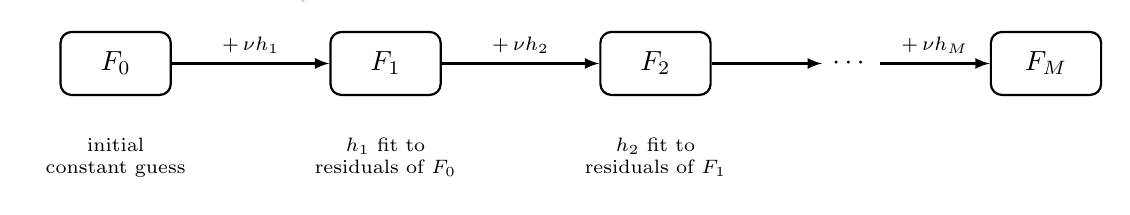
\begin{tikzpicture}[>=latex,thick,node distance=2.0cm]
        \node[draw,rounded corners,minimum width=1.4cm,minimum height=0.8cm] (f0) {$F_0$};
        \node[draw,rounded corners,minimum width=1.4cm,minimum height=0.8cm,right=of f0] (f1) {$F_1$};
        \node[draw,rounded corners,minimum width=1.4cm,minimum height=0.8cm,right=of f1] (f2) {$F_2$};
        \node[right=1.4cm of f2] (dots) {$\cdots$};
        \node[draw,rounded corners,minimum width=1.4cm,minimum height=0.8cm,right=1.4cm of dots] (fm) {$F_M$};
        \draw[->] (f0) -- node[above,font=\scriptsize] {$+\,\nu h_1$} (f1);
        \draw[->] (f1) -- node[above,font=\scriptsize] {$+\,\nu h_2$} (f2);
        \draw[->] (f2) -- (dots);
        \draw[->] (dots) -- node[above,font=\scriptsize] {$+\,\nu h_M$} (fm);
        \node[below=0.4cm of f0,font=\scriptsize,align=center,text width=2.0cm] {initial\\constant guess};
        \node[below=0.4cm of f1,font=\scriptsize,align=center,text width=2.4cm] {$h_1$ fit to\\residuals of $F_0$};
        \node[below=0.4cm of f2,font=\scriptsize,align=center,text width=2.4cm] {$h_2$ fit to\\residuals of $F_1$};
    \end{tikzpicture}
\end{lrbox}
\ifdim\wd\bookmeasuredbox<0.65\linewidth
\setlength{\bookcapwidth}{0.65\linewidth}
\else
\setlength{\bookcapwidth}{\wd\bookmeasuredbox}
\fi
\ffigbox[\bookcapwidth]{
\usebox{\bookmeasuredbox}
}{
    \caption{Gradient boosting as a sequential chain of shrunken trees, each fit to correct the previous stage's residuals.}
    \label{fig:boosting_sequence}
}
\end{figure}

In finance, such models are widely used for default prediction, credit scoring, and fraud detection. They can also be used to estimate the importance of variables, which can be useful for understanding which features drive a prediction. However, they are not automatically more reliable than simpler models. A tree-based model can still overfit, especially when the data are noisy or when the time structure is ignored during cross-validation. Careful validation, along the lines discussed in Section~\ref{sec:overfitting-section} and using walk-forward schemes rather than random splits, remains essential.

Table~\ref{tab:bagging_vs_boosting} summarizes the key differences between the two ensembling strategies introduced above, since they are easily confused despite solving different problems.

\begin{table}[htbp]
\centering
\caption{Bagging (random forests) versus boosting (gradient-boosted trees)}
\label{tab:bagging_vs_boosting}
\begin{tabular}{p{2.8cm}p{5.0cm}p{5.0cm}}
\toprule
 & Bagging (e.g., random forest) & Boosting (e.g., gradient boosting\index{gradient boosting}) \\
\midrule
Trees built & In parallel, independently & Sequentially, each correcting the last \\
Primarily reduces & Variance & Bias \\
Base learner & Deep, low-bias trees & Shallow, high-bias trees \\
Overfitting risk & Lower, more robust to noise & Higher, requires careful tuning \\
Typical use case & Robust baseline with minimal tuning & Squeezing out maximum predictive accuracy \\
\bottomrule
\end{tabular}
\end{table}

Neither approach dominates the other in every setting, but the difference in overfitting risk is a genuinely important practical consideration in finance: a gradient-boosted model with many trees and a small learning rate can achieve very low training error, and following the walk-forward validation discipline of Chapter 7 rather than a random split is especially important for catching overfitting before it reaches production.

\section{Naive Bayes: A Probabilistic Classifier}\index{Naive Bayes: A Probabilistic Classifier}

Chapter 1 introduced Bayes' theorem\index{Bayes' theorem} using a fraud-detection example; naive Bayes turns that same idea into a full classification algorithm. Given features $x_1, \ldots, x_p$, it estimates the probability of each class $k$ using Bayes' theorem,
\begin{equation*}
\Pr(y=k \mid x_1, \ldots, x_p) \propto \Pr(y=k) \prod_{j=1}^p \Pr(x_j \mid y=k),
\end{equation*}
and predicts whichever class has the highest resulting probability. The ``naive'' assumption is that the features are conditionally independent given the class, which is rarely exactly true (a firm's leverage and interest coverage, for example, are clearly related) but often works well enough in practice to be a fast, effective baseline, particularly for text classification tasks such as the sentiment analysis introduced in Chapter 14, where the features are word counts or word presence indicators and the independence assumption, while still technically false, distorts the result less than it might for tightly coupled financial ratios. Naive Bayes trains almost instantly even on large datasets, since fitting it only requires estimating simple frequency-based probabilities rather than solving an optimization problem like gradient descent, which makes it a useful quick baseline to compare against before investing in a more sophisticated model.

For text classification specifically, where each feature $x_j$ is a count of how often a particular word appears, the individual probabilities $\Pr(x_j \mid y=k)$ are most naturally estimated directly from training-data word frequencies, the fraction of class $k$'s total word count occupied by word $x_j$. This raw frequency estimate has a serious practical flaw: any word that simply never happens to appear in class $k$'s training documents receives an estimated probability of exactly zero, and because the naive Bayes score is a \emph{product} across all features, a single zero-probability word forces the entire product to zero regardless of how strongly every other word favors that class, an artifact of a small training sample rather than genuine evidence the class is impossible. Laplace smoothing\index{Laplace smoothing} (also called add-one smoothing) fixes this by adding a small constant to every count before normalizing,
\begin{equation*}
\Pr(x_j \mid y=k) = \frac{\text{count}(x_j, k) + 1}{\text{count}(k) + V},
\end{equation*}
where $\text{count}(x_j,k)$ is how many times word $x_j$ appeared across class $k$'s training documents, $\text{count}(k)$ is the total word count across those same documents, and $V$ is the vocabulary size, the number of distinct words being counted. Adding one to the numerator guarantees every word receives a strictly positive probability even if it was never observed in that class's training data, while adding $V$ to the denominator keeps the resulting probabilities properly normalized, summing to one across the vocabulary. Chapter 14's 10-K risk-factor classifier applies exactly this correction.

\section{Clustering and Dimensionality Reduction}\index{Clustering and Dimensionality Reduction}

Not all machine learning tasks involve predicting a known outcome. Sometimes the goal is to understand structure in a large set of assets or transactions. Suppose a portfolio manager has a spreadsheet of a few hundred holdings and no label telling her which ones behave similarly; she would like an algorithm that groups them automatically, purely from their measured characteristics, rather than sorting them by eye. $K$-means clustering\index{K-means clustering} partitions observations into $K$ groups by minimizing the within-cluster sum of squared distances to each group's center,
\begin{equation*}
\arg\min_{\{S_k\}} \sum_{k=1}^K \sum_{x_i \in S_k} \|x_i - \mu_k\|^2, \qquad \mu_k = \frac{1}{|S_k|}\sum_{x_i \in S_k} x_i,
\end{equation*}
where $S_k$ denotes the set of observations assigned to cluster $k$ and $\mu_k$ is that cluster's center, the mean of its assigned points. This groups similar observations together, for example firms with similar financial profiles or trading accounts with similar behavior. Principal component analysis (PCA)\index{Principal Component Analysis (PCA)} is the standard dimensionality-reduction method: it finds the direction $w$ (with $\|w\|=1$) that maximizes the variance of the projected data, $\arg\max_w \text{Var}(Xw)$, then finds the next such direction orthogonal to the first, and so on. In finance, PCA applied to a panel of asset returns often reveals that a small number of components, frequently interpretable as a broad market factor followed by sector or style factors, explain the large majority of the total variance.

These approaches are especially useful when the analyst faces high-dimensional data and wants to uncover latent structure. For instance, a portfolio manager may want to understand whether returns are driven by a few common factors or by many idiosyncratic sources, a question addressed more fully in Chapter 10. A fraud analyst may want to identify clusters of unusual behavior that deserve closer investigation. In both cases, unsupervised learning can provide a valuable first step before more targeted modeling.

To make $K$-means concrete, consider four firms described by two features, leverage and profit margin (both scaled to lie between 0 and 1):
\begin{align*}
F_1 &= (0.20, 0.30), & F_2 &= (0.30, 0.25), \\
F_3 &= (0.80, 0.05), & F_4 &= (0.90, 0.10).
\end{align*}
Initializing two cluster centers at $F_1$ and $F_4$, the algorithm alternates between two steps: assign each point to its nearest center, then recompute each center as the mean of its assigned points. In this example, $F_1$ and $F_2$ (both low leverage, higher margin) are closest to the first center, while $F_3$ and $F_4$ (both high leverage, low margin) are closest to the second, giving updated centers $\mu_1 = (0.25, 0.275)$ and $\mu_2 = (0.85, 0.075)$. Recomputing distances with these updated centers does not change any point's assignment, so the algorithm has converged after a single update: the data naturally separates into a ``low-leverage, higher-margin'' group and a ``high-leverage, low-margin'' group, without ever being told what leverage or margin mean, purely from the geometry of the two features. Figure~\ref{fig:kmeans_example} shows the four firms, the initial centers, and the updated centers $\mu_1$ and $\mu_2$ together.

\begin{figure}[htbp]
\centering
\begin{lrbox}{\bookmeasuredbox}
    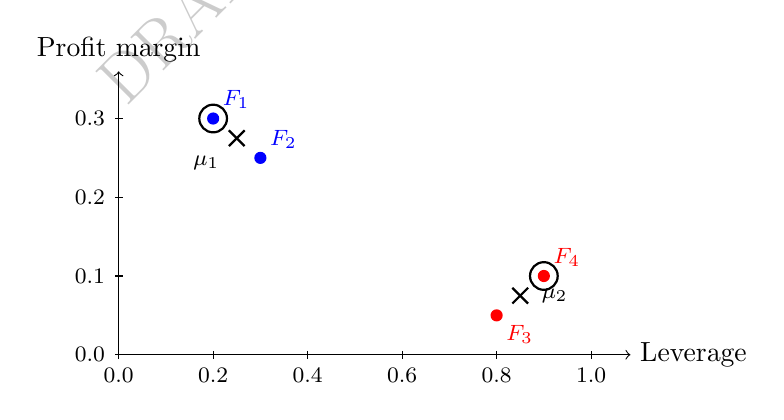
\begin{tikzpicture}[scale=1.0]
        \draw[->] (0,0) -- (6.5,0) node[right] {Leverage};
        \draw[->] (0,0) -- (0,3.6) node[above] {Profit margin};
        \foreach \x/\lbl in {0/0.0, 1.2/0.2, 2.4/0.4, 3.6/0.6, 4.8/0.8, 6.0/1.0} {
            \draw (\x,0.05) -- (\x,-0.05) node[below,font=\footnotesize] {\lbl};
        }
        \foreach \y/\lbl in {0/0.0, 1.0/0.1, 2.0/0.2, 3.0/0.3} {
            \draw (0.05,\y) -- (-0.05,\y) node[left,font=\footnotesize] {\lbl};
        }
        \fill[blue] (1.2,3.0) circle (2.2pt) node[above right,font=\footnotesize] {$F_1$};
        \fill[blue] (1.8,2.5) circle (2.2pt) node[above right,font=\footnotesize] {$F_2$};
        \fill[red] (4.8,0.5) circle (2.2pt) node[below right,font=\footnotesize] {$F_3$};
        \fill[red] (5.4,1.0) circle (2.2pt) node[above right,font=\footnotesize] {$F_4$};
        \draw[black,thick] (1.2,3.0) circle (5pt);
        \draw[black,thick] (5.4,1.0) circle (5pt);
        \draw[black,thick] (1.4,2.65) -- (1.6,2.85);
        \draw[black,thick] (1.4,2.85) -- (1.6,2.65);
        \node[below left,font=\footnotesize] at (1.4,2.65) {$\mu_1$};
        \draw[black,thick] (5.0,0.65) -- (5.2,0.85);
        \draw[black,thick] (5.0,0.85) -- (5.2,0.65);
        \node[right,font=\footnotesize] at (5.25,0.75) {$\mu_2$};
    \end{tikzpicture}
\end{lrbox}
\ifdim\wd\bookmeasuredbox<0.65\linewidth
\setlength{\bookcapwidth}{0.65\linewidth}
\else
\setlength{\bookcapwidth}{\wd\bookmeasuredbox}
\fi
\ffigbox[\bookcapwidth]{
\usebox{\bookmeasuredbox}
}{
    \caption{The $K$-means example: four firms in leverage/profit-margin space, with the initial centers (circled) and the updated centers $\mu_1$ and $\mu_2$.}
    \label{fig:kmeans_example}
}
\end{figure}

\section{Neural Networks and Deep Learning in Finance}\index{Neural Networks and Deep Learning in Finance}

Suppose an analyst suspects that default risk depends on leverage and profitability not through any simple additive combination, but through some more intricate interaction between the two that is too complex to write down as a specific nonlinear formula in advance, and wants a model flexible enough to learn whatever that relationship turns out to be directly from data, rather than committing in advance to a particular functional form the way linear or logistic regression do. Neural networks represent another major class of machine learning methods, built for exactly this kind of unspecified nonlinearity. A simple feedforward network with one hidden layer computes
\begin{equation*}
\hat y = \sigma_2\big(W_2\, \sigma_1(W_1 x + b_1) + b_2\big),
\end{equation*}
where $W_1, b_1, W_2, b_2$ are learned weight matrices and bias vectors, and $\sigma_1, \sigma_2$ are nonlinear activation functions, such as the rectified linear unit $\text{ReLU}(z) = \max(0,z)$ for hidden layers or the sigmoid function for a binary output layer. Stacking more such layers produces a deep network. The weights are learned by minimizing a loss function (mean squared error for regression, log-loss for classification) using gradient descent, with gradients computed efficiently via backpropagation\index{backpropagation}, an efficient algorithm for computing the gradient of the loss with respect to every weight in the network by applying the chain rule layer by layer from the output back to the input.

A small numerical example makes the forward pass (computing a prediction from an input) concrete. Suppose a network has two inputs, a hidden layer with two ReLU units, and a single sigmoid output, with weights
\begin{equation*}
W_1 = \begin{pmatrix} 0.4 & -0.2 \\ 0.1 & 0.3 \end{pmatrix}, \quad b_1 = \begin{pmatrix} 0.05 \\ -0.1 \end{pmatrix}, \quad W_2 = \begin{pmatrix} 0.6 & -0.5 \end{pmatrix}, \quad b_2 = 0.1.
\end{equation*}
For an input $x = (1.0, 0.5)$, the hidden layer's pre-activation values are $W_1 x + b_1 = (0.35, 0.15)$, and since both are already positive, the ReLU activation leaves them unchanged: $h = (0.35, 0.15)$. The output layer's pre-activation is $W_2 h + b_2 = 0.6(0.35) - 0.5(0.15) + 0.1 = 0.235$, and applying the sigmoid function gives the final prediction $\hat y = 1/(1+e^{-0.235}) \approx 0.558$.

Every one of the millions of parameters in a modern deep network is used in exactly this way, matrix multiplications and elementwise nonlinearities, repeated layer after layer; what makes deep learning powerful is not any single computation's complexity but the ability to learn, via backpropagation and gradient descent, weight values across many layers that jointly capture useful nonlinear structure in the data. Figure~\ref{fig:toy_feedforward_network} lays out this exact network: two input neurons feed forward into two ReLU hidden neurons, which feed forward into a single sigmoid output neuron, with every edge and bias labeled with the weight values above and every neuron labeled with the value it computes.

\subsection*{A Worked Example: Backpropagation, One Layer at a Time}

Section 6.5 introduced gradient descent for a single-layer linear regression, where the gradient of the loss with respect to each parameter could be written down directly. A multi-layer network needs the chain rule to propagate a gradient backward through each layer in turn, backpropagation, and the same toy network above makes every step concrete. Suppose this network is being trained as a classifier and the true label for input $x=(1.0,0.5)$ is $y=1$ (a positive case, using the log-loss $L=-[y\ln\hat y+(1-y)\ln(1-\hat y)]$ standard for classification). A well-known simplification, for exactly this pairing of sigmoid output and log-loss, is that the gradient of the loss with respect to the output layer's pre-activation $z_2$ collapses to simply $\hat y - y$:
\begin{equation*}
\frac{\partial L}{\partial z_2} = \hat y - y = 0.5585 - 1 = -0.4415.
\end{equation*}
Backpropagation now works backward one layer at a time, applying the chain rule at each step. The output layer's weights and bias receive
\begin{equation*}
\frac{\partial L}{\partial W_2} = \frac{\partial L}{\partial z_2}\, h^\top = -0.4415\,(0.35,\ 0.15) = (-0.1545,\ -0.0662), \qquad \frac{\partial L}{\partial b_2} = \frac{\partial L}{\partial z_2} = -0.4415.
\end{equation*}
To continue backward into the hidden layer, the gradient must first pass through $W_2$ to reach $h$, then through the ReLU activation to reach the hidden layer's pre-activations $z_1$:
\begin{equation*}
\frac{\partial L}{\partial h} = \frac{\partial L}{\partial z_2}\,W_2 = -0.4415\,(0.6,\ -0.5) = (-0.2649,\ 0.2208), \qquad \frac{\partial L}{\partial z_1} = \frac{\partial L}{\partial h} \odot \text{ReLU}'(z_1),
\end{equation*}
where $\text{ReLU}'(z)=1$ if $z>0$ and $0$ otherwise, and $\odot$ denotes elementwise multiplication; since both hidden pre-activations ($0.35$ and $0.15$) are positive, $\text{ReLU}'(z_1)=(1,1)$ here and $\partial L/\partial z_1$ passes through unchanged. Finally, the first layer's weights and bias receive
\begin{equation*}
\frac{\partial L}{\partial W_1} = \frac{\partial L}{\partial z_1}\,x^\top = \begin{pmatrix} -0.2649 \\ 0.2208 \end{pmatrix}(1.0,\ 0.5) = \begin{pmatrix} -0.2649 & -0.1325 \\ 0.2208 & 0.1104 \end{pmatrix}, \qquad \frac{\partial L}{\partial b_1} = \frac{\partial L}{\partial z_1} = (-0.2649,\ 0.2208).
\end{equation*}
Every one of these four gradients was obtained purely by repeated application of the chain rule, working from the loss backward to the output layer, then backward again through the hidden layer, never once needing to re-derive the forward pass from scratch; this reuse of intermediate quantities computed once, moving backward, is precisely what makes backpropagation efficient enough to train networks with millions of parameters, rather than the (computationally infeasible) alternative of perturbing each weight individually and re-running the entire forward pass to estimate its gradient numerically.

A single gradient descent step with learning rate $\eta=0.1$, exactly the update rule Section 6.5 introduced, moves every parameter a small step opposite its gradient, $W_2 \leftarrow W_2 - \eta\,\partial L/\partial W_2$ and likewise for $b_2$, $W_1$, and $b_1$, nudging the network's prediction for this particular example fractionally closer to the target $y=1$, and repeating this update across many training examples and many iterations is, in its entirety, how a deep network's weights are actually learned.

\begin{figure}[htbp]
\centering
\begin{lrbox}{\bookmeasuredbox}
    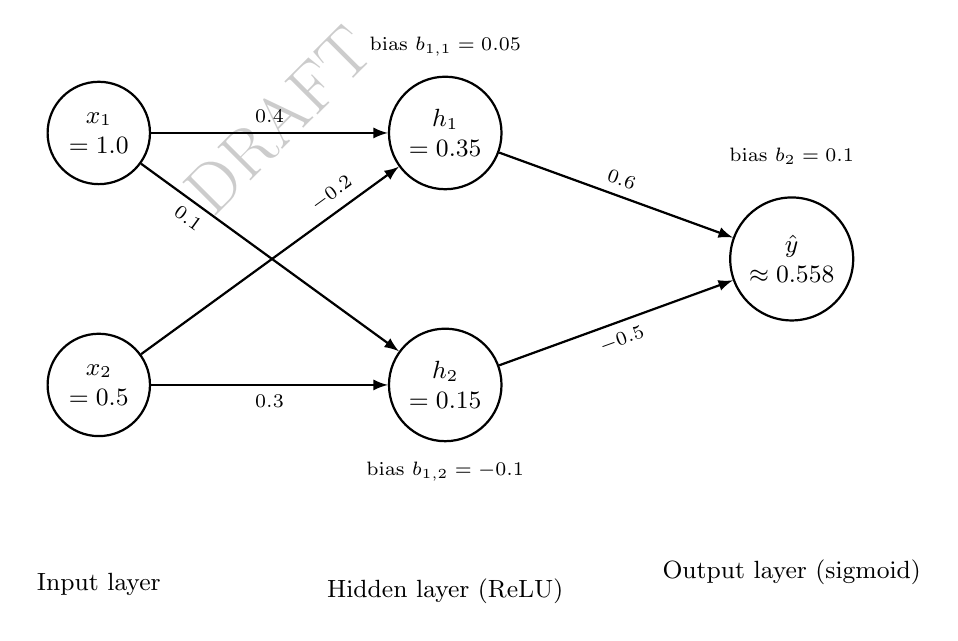
\begin{tikzpicture}[>=latex,thick,
        neuron/.style={draw,circle,minimum size=1.3cm,align=center,font=\small},
        biaslabel/.style={font=\scriptsize,align=center}]
        \node[neuron] (x1) at (0,1.6) {$x_1$\\$=1.0$};
        \node[neuron] (x2) at (0,-1.6) {$x_2$\\$=0.5$};
        \node[neuron] (h1) at (4.4,1.6) {$h_1$\\$=0.35$};
        \node[neuron] (h2) at (4.4,-1.6) {$h_2$\\$=0.15$};
        \node[neuron] (y) at (8.8,0) {$\hat y$\\$\approx 0.558$};

        \draw[->] (x1) -- node[above,sloped,font=\scriptsize]{$0.4$} (h1);
        \draw[->] (x1) -- node[below,sloped,font=\scriptsize,pos=0.22]{$0.1$} (h2);
        \draw[->] (x2) -- node[above,sloped,font=\scriptsize,pos=0.78]{$-0.2$} (h1);
        \draw[->] (x2) -- node[below,sloped,font=\scriptsize]{$0.3$} (h2);
        \draw[->] (h1) -- node[above,sloped,font=\scriptsize]{$0.6$} (y);
        \draw[->] (h2) -- node[below,sloped,font=\scriptsize]{$-0.5$} (y);

        \node[biaslabel] at (4.4,2.7) {bias $b_{1,1}=0.05$};
        \node[biaslabel] at (4.4,-2.7) {bias $b_{1,2}=-0.1$};
        \node[biaslabel] at (8.8,1.3) {bias $b_2=0.1$};

        \node[font=\small,below=1.6cm of x2] {Input layer};
        \node[font=\small,below=1.6cm of h2] {Hidden layer (ReLU)};
        \node[font=\small,below=2.9cm of y] {Output layer (sigmoid)};
    \end{tikzpicture}
\end{lrbox}
\ifdim\wd\bookmeasuredbox<0.65\linewidth
\setlength{\bookcapwidth}{0.65\linewidth}
\else
\setlength{\bookcapwidth}{\wd\bookmeasuredbox}
\fi
\ffigbox[\bookcapwidth]{
\usebox{\bookmeasuredbox}
}{
    \caption{The toy feedforward network worked through above. Chapter 16 revisits it to verify LIME and integrated-gradients explanations against its exact analytical gradient.}
    \label{fig:toy_feedforward_network}
}
\end{figure}

In finance, neural networks have been used for forecasting, option pricing, time series modeling, and text analysis. The appeal of deep learning is that it can automatically learn useful nonlinear representations from raw data, reducing the need for hand-crafted features. However, neural networks are not a magic solution. They often require substantial data, careful tuning of architecture and learning rate, and strong regularization (such as dropout or weight decay, which is mathematically equivalent to the ridge penalty introduced earlier) to avoid overfitting. They may also be more difficult to interpret than a linear model or a single decision tree, which matters when the model influences real-world, and sometimes regulated, decisions. For this reason, deep learning is often most useful when paired with domain knowledge and robust validation practices. A neural network that performs well in a laboratory setting may still fail in production if the data environment shifts or if the model is not monitored properly.

\section{Challenges of Machine Learning in Finance}

Several challenges make financial applications of machine learning harder than many textbook demonstrations suggest.

\textbf{Low signal-to-noise ratio.} Financial returns are dominated by noise relative to the size of any genuine predictive signal, unlike many image or language tasks where the target is essentially deterministic given the input. An $R^2$ of a few percent can be economically meaningful for return prediction, whereas the same $R^2$ would be considered a failure in the clean regression example of Section~\ref{sec:regression-example}.

\textbf{Non-stationarity.} The statistical relationships a model learns can change as markets evolve, as regulation changes, or as other participants adapt their own strategies. A model is effectively trained on the past while being asked to perform in a future that may not resemble it, which is a much harder problem than the standard machine learning assumption that training and test data are drawn from the same distribution.

\textbf{Multiple testing and backtest overfitting.} When researchers try many features, model specifications, or trading rules and report only the best-performing one, the reported performance is biased upward, sometimes dramatically. This is closely related to the overfitting problem in Section~\ref{sec:overfitting-section}, but it operates across an entire research process rather than within a single model fit, and it is one of the most persistent sources of disappointing live performance after a promising backtest.

\textbf{Imbalanced outcomes.} Events such as default, fraud, or market crashes are rare relative to normal outcomes. A classifier that simply predicts ``no event'' can achieve high accuracy while being useless, which is why precision, recall, and related metrics from Section~\ref{sec:classification-example} matter more than accuracy in these settings. Practical remedies include resampling the training data (oversampling the rare class or undersampling the common one), assigning a higher misclassification cost to the rare class during training, and choosing a classification threshold explicitly based on the relative costs of false positives and false negatives for the specific decision at hand, rather than defaulting to the conventional 0.5 cutoff, which implicitly assumes the two types of error are equally costly.

\textbf{Interpretability and regulatory scrutiny.} Many financial applications, particularly credit decisions, are subject to regulation requiring that decisions be explainable to the affected individual and auditable by a regulator. This constrains the use of some highly flexible models, such as a large ensemble or a deep neural network, or requires supplementing them with explanation methods, a topic developed further in Chapter 16.

\textbf{Feedback and reflexivity.} Unlike physical systems, financial markets can react to the presence of a successful model: if a profitable pattern becomes known and widely traded, the trading activity itself can erode or eliminate the pattern. This means past predictive power is not simply a static property of the data, but can be altered by the deployment of the model itself.

\textbf{Hyperparameter and model-selection overfitting.} Section 6.11's grid-search workflow, if applied carelessly, is itself a source of overfitting: searching over many hyperparameter combinations or model families and reporting only the best cross-validated result inflates the reported performance in exactly the same way as the multiple-testing problem above, just one level removed from the original features and trading rules.

\textbf{Computational cost at scale.} Some of the most powerful techniques in this chapter, an exhaustive hyperparameter grid search, a large gradient-boosted ensemble, a deep neural network, can be computationally expensive to train and retrain, which matters in finance because models often need to be refit frequently (daily or even intraday) to stay current with a non-stationary market, creating a real engineering constraint on top of the statistical ones.

These challenges do not make machine learning inapplicable to finance; they make careful validation, economically grounded evaluation, and ongoing monitoring non-negotiable parts of any deployment, rather than optional extras.

\section{Key Takeaways}

Machine learning offers valuable tools for prediction, classification, and pattern discovery in finance, but its power must be balanced with caution. The regression and classification examples in this chapter showed exactly how the standard formulas, ordinary least squares, logistic regression, the confusion matrix, and $R^2$, are computed, so that later chapters can build on precise foundations rather than vague intuition. Overfitting, unstable relationships, and shifting regimes all threaten performance in real-world settings, and the bias-variance decomposition gives a precise vocabulary for understanding why. The most successful applications combine statistical learning with domain knowledge, careful validation, and a clear understanding of the financial decision being made.

This chapter also introduced a genuine diversity of algorithmic approaches, parametric models fit by a closed-form solution (linear regression) or by gradient descent (logistic regression and, later, neural networks), non-parametric models that reason directly from stored examples (KNN), margin-based geometric classifiers (SVM), probabilistic classifiers built directly on Bayes' theorem (naive Bayes), and ensembles of simple trees combined either in parallel to reduce variance (random forests) or sequentially to reduce bias (gradient boosting), and it is worth remembering that no single one of these is universally best. The right choice depends on the size and structure of the data, the importance of interpretability (Chapter 16 returns to this directly), and the computational constraints of the deployment setting, which is exactly why Section 6.11's disciplined, cross-validated approach to model and hyperparameter selection matters as much as knowing the algorithms themselves.

\section{Suggested Exercises}

\begin{enumerate}
    \item Using the data in Table~\ref{tab:credit_spread_data}, verify by hand that $\hat\beta_1 = 47$ and $\hat\beta_0 = 20$, and compute the fitted spread for a firm with debt/EBITDA of 4.5.
    \item Add a sixth observation, debt/EBITDA of 7 and a credit spread of 500 bps, to Table~\ref{tab:credit_spread_data}, refit the regression, and discuss how much the slope and $R^2$ change. What does this reveal about the sensitivity of OLS to outliers?
    \item Using Table~\ref{tab:confusion_data}, suppose the lender lowers its classification threshold so that applicant 5 is now also predicted to default. Recompute the confusion matrix and all five metrics, and discuss how precision and recall trade off against each other.
    \item Explain the difference between supervised and unsupervised learning, giving one financial example of each that is not already used in the chapter.
    \item Derive, in your own words, why a ridge penalty with a very large $\lambda$ drives all coefficients toward zero, and explain what this implies about the bias and variance of the resulting model.
    \item Describe the bias-variance tradeoff using the formal decomposition in Section~\ref{sec:bias-variance}, and relate each of the three terms to a specific row of Table~\ref{tab:overfitting_stylized}.
    \item Why is walk-forward validation generally preferred over random $k$-fold cross-validation for financial time series?
    \item Discuss one reason a model that performs well in-sample or in a backtest may fail out of sample or in live trading, drawing on at least two of the challenges described in Section 6.19 (``Challenges of Machine Learning in Finance'').
    \item Starting from $\beta_0=\beta_1=0$, manually compute the first gradient descent update (Section~\ref{sec:gradient-descent}) for the credit-spread data using a learning rate of $\eta=0.02$ instead of $0.01$, and compare the resulting $(\beta_0,\beta_1)$ to the first iteration shown in Table~\ref{tab:gradient_descent}.
    \item Using Table~\ref{tab:knn_data}, classify a new applicant with a debt-to-income ratio of 22\% and 6 years of credit history using $k=1$ and again using $k=5$, and explain why the two predictions differ.
    \item Explain, in your own words, why a wider margin in a support vector machine is generally associated with better generalization to new data, drawing an analogy to the bias-variance tradeoff.
    \item Choose one hyperparameter from any model in this chapter (for example, $\lambda$, $k$, or the number of boosting trees) and describe a grid of candidate values you would try, along with why searching too wide a grid could itself introduce overfitting risk, using Section 6.11 and Section 6.19's discussion of model-selection overfitting.
    \item Explain why the naive independence assumption in naive Bayes is more clearly violated for the financial-ratio features used elsewhere in this chapter than for the word-count features used in text classification, and discuss whether you would still expect naive Bayes to be a reasonable baseline for a financial application.
    \item Using this chapter's maximum-margin example, suppose a fifth point is added at $x=3.5$ belonging to the ``low-risk'' class. Compute its functional margin under the original hyperplane ($w=1$, $b=-3$), explain why this point must become a new support vector, and recompute the resulting hyperplane and margin width.
    \item Using this chapter's ridge-versus-lasso worked example, explain in your own words why lasso's exact zero for the spurious feature's coefficient is a direct consequence of the penalty term's shape (a kink at zero), rather than simply a coincidence of this particular dataset, and describe what would need to be true of ridge's penalty for it to ever produce an exactly zero coefficient.
    \item Using this chapter's backpropagation worked example, recompute $\partial L/\partial z_2$, $\partial L/\partial W_2$, and $\partial L/\partial b_2$ if the true label were $y=0$ instead of $y=1$ (all forward-pass values unchanged), and explain in words why the sign of every downstream gradient flips as a result.
    \item \textbf{Challenge (real data).} Download the UCI Bank Marketing dataset (a Portuguese bank's telemarketing campaign, roughly 45,000 client contacts, with features such as age, job, account balance, and prior campaign outcomes, and a binary label for whether the client subscribed to a term deposit). (a) Fit both a logistic regression and a $k$-nearest-neighbors classifier (trying at least three values of $k$) to predict subscription on a held-out test split, and compare their accuracy, precision, and recall. (b) Using Section~\ref{sec:bias-variance}'s bias-variance framework, explain which of your $k$ values appears to underfit and which appears to overfit, based on how training and test accuracy diverge. (c) This dataset's subscription rate is only around $11\%$, far from the roughly balanced toy examples used elsewhere in this chapter; discuss, referencing this chapter's overfitting and validation material, why a model that reports $89\%$ accuracy on this dataset could still be practically useless to the bank's marketing team.
\end{enumerate}

\section{Further Reading}

\begin{itemize}
    \item Hastie, Tibshirani, and Friedman, \emph{The Elements of Statistical Learning}. The standard advanced reference for the statistical theory behind essentially every model in this chapter, including a much more rigorous treatment of the bias-variance decomposition and regularization.
    \item Murphy, \emph{Machine Learning: A Probabilistic Perspective}. A thorough, probability-first treatment that develops naive Bayes, logistic regression, and neural networks within a unified Bayesian framework, extending the Bayes' theorem introduction from Chapter 1.
    \item James et al., \emph{An Introduction to Statistical Learning}. A more accessible companion to Hastie, Tibshirani, and Friedman, with the same authors and worked examples in R and Python; a good starting point before attempting the more mathematically demanding treatment.
    \item Hull et al., \emph{Machine Learning in Business: An Introduction to the World of Data Science}. A business- and finance-oriented introduction to many of this chapter's models, by the same Hull whose derivatives and risk-management texts are cited in Chapters 1, 3, 5, 8, and 9, with less formal derivation and more emphasis on practical business use cases than the theory-first references above.
    \item de Prado, \emph{Advances in Financial Machine Learning}. Focuses specifically on the financial-data pitfalls emphasized throughout this chapter, backtest overfitting, walk-forward validation, and feature construction for financial time series, in far greater depth than a single chapter allows.
    \item Cristianini and Shawe-Taylor, \emph{An Introduction to Support Vector Machines}. A focused treatment of the margin-maximization and kernel-trick ideas introduced only briefly in this chapter.
\end{itemize}

\end{document}
